\documentclass[a4paper]{article}
\usepackage{ctex}
\usepackage[affil-it]{authblk}
\usepackage[backend=bibtex,style=numeric]{biblatex}
\usepackage{amsmath,amsthm,amssymb,amsfonts}
\usepackage{graphicx}
\usepackage{bm}

\usepackage{geometry}
\geometry{margin=1.5cm, vmargin={0pt,1cm}}
\setlength{\topmargin}{-1cm}
\setlength{\paperheight}{29.7cm}
\setlength{\textheight}{25.3cm}

\addbibresource{citation.bib}

\begin{document}
% =================================================
\title{微分方程数值解 2026 春夏作业八}

\author{曾申昊 3220100701
  \thanks{邮箱: \texttt{3097714673@qq.com}
                            \texttt{或} \texttt{3220100701@zju.edu.cn}}}
\affil{浙江大学}

\date{更新时间: \today}

\maketitle

% ============================================
\section*{Exercise 14.13}

\par Crank-Nicolson method 的离散格式为
\begin{equation}
    \frac{U_{i}^{n+1}-U_{i}^{n}}{k} 
    = \frac{\nu}{2h^2}
    \left(
        U_{i-1}^{n}-2U_{i}^{n}+U_{i+1}^{n}
        +U_{i-1}^{n+1}-2U_{i}^{n+1}+U_{i+1}^{n+1}
    \right)
\end{equation}
\par 以及 Dirichlet 边界条件
\begin{equation}
    \begin{cases}
        u(0,t)=g_0(t)\qquad \text{on } {0} \times (0,T)\\
        u(1,t)=g_1(t)\qquad \text{on } {1} \times (0,T)
    \end{cases}
\end{equation}
\par 写成矩阵形式为
\begin{equation}
    \begin{gathered}
        U_{i}^{n+1} - \frac{k}{2}\frac{\nu}{h^2}
        \left(
            U_{i-1}^{n+1}-2U_{i}^{n+1}+U_{i+1}^{n+1}
        \right)
        = U_{i}^{n} + \frac{k}{2}\frac{\nu}{h^2}
        \left(
            U_{i-1}^{n}-2U_{i}^{n}+U_{i+1}^{n}
        \right)\\
        \left(
            I - \frac{k}{2}A
        \right)\mathbf{U}^{n+1} = \left(
            I + \frac{k}{2}A
        \right)\mathbf{U}^{n} + \mathbf{b}^{n}
    \end{gathered}
\end{equation}
\par 其中
\begin{equation}
    A = \frac{\nu}{h^2}
    \begin{bmatrix}
        -2 & 1 & 0 & \cdots & 0\\
        1 & -2 & 1 & \cdots & 0\\
        0 & 1 & -2 & \cdots & 0\\
        \vdots & \vdots & \vdots & \ddots & \vdots\\
        0 & 0 & 0 & \cdots & -2
    \end{bmatrix}\qquad
    \mathbf{b}^{n} = 
    \frac{k}{2}\frac{\nu}{h^2}
    \begin{bmatrix}
        g_0(t_{n+1}) + g_0(t_n)\\
        0\\
        0\\
        \vdots\\
        g_1(t_{n+1}) + g_1(t_n)
    \end{bmatrix}\qquad
    \mathbf{U}^{n} =
    \begin{bmatrix}
        U_1^{n}\\
        U_2^{n}\\
        U_3^{n}\\
        \vdots\\
        U_{m}^{n}
    \end{bmatrix}
\end{equation}

\section*{Exercise 14.28}

\par $\theta$-method 的离散格式为
\begin{equation}
    \begin{gathered}
        \frac{U_{i}^{n+1}-U_{i}^{n}}{k} 
        = \frac{\nu}{h^2}
        \left[
            (1-\theta)\left(
                U_{i-1}^{n}-2U_{i}^{n}+U_{i+1}^{n}
            \right) + \theta
            \left(
                U_{i-1}^{n+1}-2U_{i}^{n+1}+U_{i+1}^{n+1}
            \right)
        \right]\\
        \left(
            I - \theta kA
        \right)\mathbf{U}^{n+1} = \left(
            I + (1-\theta)kA
        \right)\mathbf{U}^{n} + \mathbf{b}^{n}
    \end{gathered}
\end{equation}
\par 绝对稳定要求
\begin{equation}
    \left|\frac{1+(1-\theta)k\lambda}{1-\theta k\lambda}\right|
    \leq 1
\end{equation}
\par 其中 $\lambda$ 为矩阵 $A$ 的特征值，即 
$\lambda_p = -\dfrac{4\nu}{h^2}\sin^2\left(\dfrac{p\pi h}{2}\right)\leq 0$。
\par 上式等价于
\begin{equation}
    \begin{gathered}
        \left|1+(1-\theta)k\lambda\right|
        \leq \left|1-\theta k\lambda\right|\\
        \left|1+(1-\theta)k\lambda\right|^2
        \leq \left|1-\theta k\lambda\right|^2\\
        2k\lambda + (1-2\theta)k^2\lambda^2
        \leq 0\\
        2 + (1-2\theta)k\lambda
        \geq 0\\
    \end{gathered}
\end{equation}
\par 当 $\theta \in \left[\dfrac{1}{2}, 1\right]$ 时，$1-2\theta \leq 0$，所以上式恒成立。
当 $\theta \in \left[0, \dfrac{1}{2}\right]$ 时，$1-2\theta > 0$，要求
\begin{equation}
    k \leq -\frac{2}{(1-2\theta)\lambda} 
    \leq \frac{h^2}{2(1-2\theta)\nu}
\end{equation}

\section*{Exercise 14.62}

\par $L^1(h\mathbb{Z})$ 为
\begin{equation}
    L^1(h\mathbb{Z}) = \left\{
        g: h\mathbb{Z} \to \mathbb{R}
        \left|
            \sum_{j=-\infty}^{\infty}|g(jh)| < \infty
        \right.
    \right\}
\end{equation}
\par 取 $U\in L^1(h\mathbb{Z})$，做 Fourier transform 和 inverse Fourier transform，得到
\begin{equation}
    \begin{aligned}
        U(m) 
        &= \frac{1}{\sqrt{2\pi}}
        \int_{-\frac{\pi}{h}}^{\frac{\pi}{h}}
        e^{\mathbf{i}mh\xi}\hat{U}(\xi)\text{d}\xi\\
        &= \frac{1}{\sqrt{2\pi}}
        \int_{-\frac{\pi}{h}}^{\frac{\pi}{h}}
        e^{\mathbf{i}mh\xi}
        \left(\frac{h}{\sqrt{2\pi}}
            \sum_{j=-\infty}^{\infty}e^{-\mathbf{i}jh\xi}U(jh)
        \right)\text{d}\xi\\
        &= \frac{h}{2\pi}\sum_{j=-\infty}^{\infty}U(jh)
        \left(
            \int_{-\frac{\pi}{h}}^{\frac{\pi}{h}}
            e^{\mathbf{i}(m-j)h\xi}\text{d}\xi
        \right)\\
        &= \frac{h}{2\pi}\sum_{j=-\infty}^{\infty}U(jh)\delta_{mj}\left(\frac{2\pi}{h}\right)\\
        &= U(m)
    \end{aligned}
\end{equation}
\par 其中 $\delta_{mj}$ 为 Kronecker delta 函数。
$U\in L^1(h\mathbb{Z})$ 的条件是为了满足积分和求和的可交换性。

\section*{Exercise 14.69}

\par 将 fourier transform 作用于 $\theta$-method 的离散格式，得到
\begin{equation}
    \begin{gathered}
        U_{i}^{n+1} - \theta k\frac{\nu}{h^2}
        \left(
            U_{i-1}^{n+1}-2U_{i}^{n+1}+U_{i+1}^{n+1}
        \right)
        = U_{i}^{n} + (1-\theta) k\frac{\nu}{h^2}
        \left(
            U_{i-1}^{n}-2U_{i}^{n}+U_{i+1}^{n}
        \right)\\
        \frac{1}{\sqrt{2\pi}}
        \int_{-\frac{\pi}{h}}^{\frac{\pi}{h}}
        \left[
            e^{\mathbf{i}ih\xi}
            - \theta r
            \left(
                e^{\mathbf{i}(i-1)h\xi}-2e^{\mathbf{i}ih\xi}+e^{\mathbf{i}(i+1)h\xi}
            \right)
        \right]
        \hat{U}^{n+1}(\xi)\text{d}\xi\qquad\qquad\qquad\qquad\qquad\\
        \qquad\qquad\qquad\qquad\qquad=\frac{1}{\sqrt{2\pi}}
        \int_{-\frac{\pi}{h}}^{\frac{\pi}{h}}
        \left[
            e^{\mathbf{i}ih\xi}
            + (1-\theta) r
            \left(
                e^{\mathbf{i}(i-1)h\xi}-2e^{\mathbf{i}ih\xi}+e^{\mathbf{i}(i+1)h\xi}
            \right)
        \right]
        \hat{U}^{n}(\xi)\text{d}\xi\\
    \end{gathered}
\end{equation}
\par 然后可以得到 $g(h\xi)$
\begin{equation}
    \begin{aligned}
        g(h\xi)&=\frac{e^{\mathbf{i}ih\xi} + (1-\theta) r \left(e^{\mathbf{i}(i-1)h\xi} - 2e^{\mathbf{i}ih\xi} + e^{\mathbf{i}(i+1)h\xi}\right)}{e^{\mathbf{i}ih\xi} - \theta r \left(e^{\mathbf{i}(i-1)h\xi} - 2e^{\mathbf{i}ih\xi} + e^{\mathbf{i}(i+1)h\xi}\right)}\\
        &=\frac{1 - 4(1-\theta)r\sin^2\left(\frac{h\xi}{2}\right)}{1 + 4\theta r\sin^2\left(\frac{h\xi}{2}\right)}
    \end{aligned}
\end{equation}
\par 由 $\left|g(h\xi)\right|<1$ 可得稳定性条件
\begin{equation}
    \begin{gathered}
        \left|1 - 4(1-\theta)r\sin^2\left(\frac{h\xi}{2}\right)\right|
        \leq \left|1 + 4\theta r\sin^2\left(\frac{h\xi}{2}\right)\right|\\
        \left|1 - 4(1-\theta)r\sin^2\left(\frac{h\xi}{2}\right)\right|^2
        \leq \left|1 + 4\theta r\sin^2\left(\frac{h\xi}{2}\right)\right|^2\\
        -8r\sin^2\left(\frac{h\xi}{2}\right) + 16(1-2\theta)r^2\sin^4\left(\frac{h\xi}{2}\right)
        \leq 0\\
        -1 + 2(1-2\theta)r\sin^2\left(\frac{h\xi}{2}\right)
        \leq 0\\
    \end{gathered}
\end{equation}
\par 当 $\theta \in \left[\dfrac{1}{2}, 1\right]$ 时，$1-2\theta \leq 0$，所以上式恒成立。
当 $\theta \in \left[0, \dfrac{1}{2}\right]$ 时，$1-2\theta > 0$，要求
\begin{equation}
    r \leq \frac{1}{2(1-2\theta)\sin^2\left(\frac{h\xi}{2}\right)} \leq \frac{1}{2(1-2\theta)}
\end{equation}
\par 即 $k\leq \dfrac{h^2}{2(1-2\theta)\nu}$，说明时域和频域得到的稳定性条件是一致的。

\section*{Exercise 14.99}

\par Beam-Warming method 的离散格式为
\begin{equation}
    \begin{gathered}
        U_{j}^{n+1} = U_{j}^{n} - \frac{\mu}{2}
        \left(
            3U_{j}^{n}-4U_{j-1}^{n}+U_{j-2}^{n}
        \right) + \frac{\mu^2}{2}
        \left(
            U_{j}^{n}-2U_{j-1}^{n}+U_{j-2}^{n}
        \right) \qquad \text{if } a \geq 0\\
        U_{j}^{n+1} = U_{j}^{n} - \frac{\mu}{2}
        \left(
            -3U_{j}^{n}+4U_{j+1}^{n}-U_{j+2}^{n}
        \right) + \frac{\mu^2}{2}
        \left(
            U_{j}^{n}-2U_{j+1}^{n}+U_{j+2}^{n}
        \right) \qquad \text{if } a < 0\\
    \end{gathered}
\end{equation}
\par 以 $a \geq 0$ 为例，计算 $\tau(x,t)$ 
\begin{equation}
    \begin{aligned}
        \tau(x,t) &= \frac{u(x,t+k)-u(x,t)}{k} + a\frac{3u(x,t)-4u(x-h,t)+u(x-2h,t)}{2h} - ka^2\frac{u(x,t)-2u(x-h,t)+u(x-2h,t)}{2h^2}\\
        &= \left[
            u_t + \frac{1}{2}ku_{tt}+\frac{1}{6}k^2u_{ttt} + O(k^3)
        \right]\\
        &\qquad + \frac{a}{2h}\left[
            3u -4\left(u-hu_x+\frac{1}{2}h^2u_{xx}\right)
            +\left(u-2hu_x+\frac{1}{2}(2h)^2u_{xx}\right)
            + O(h^3)
        \right]\\
        &\qquad- \frac{ka^2}{2h^2}\left[
            u -2\left(u-hu_x+\frac{1}{2}h^2u_{xx}-\frac{1}{6}h^3u_{xxx}\right)
            +\left(u-2hu_x+\frac{1}{2}(2h)^2u_{xx}-\frac{1}{6}(2h)^3u_{xxx}\right)
            + O(h^4)
        \right]\\
        &= \left[
            u_t+\frac{1}{2}ku_{tt}+\frac{1}{6}k^2u_{ttt} + O(k^3)
        \right]
        +\frac{a}{2h}\left[
            2hu_x + O(h^3)
        \right]
        -\frac{ka^2}{2h^2}\left[
            h^2u_{xx}-h^3u_{xxx}+O(h^4)   
        \right]\\
        &= \left[
            u_t + au_x
        \right]
        +\left[
            \frac{1}{2}ku_{tt} - \frac{1}{2}ka^2u_{xx}
        \right]
        + O(k^2+h^2+kh)\\
        &= O(k^2+h^2)
    \end{aligned}
\end{equation}
\par 该方法在时间和空间上都是二阶精度的。

\section*{Exercise 14.100}

\par 同样以 $a \geq 0$ 为例
\begin{equation}
    U_{j}^{n+1}
    = U_{j}^{n} - \frac{\mu}{2}
        \left(
            3U_{j}^{n}-4U_{j-1}^{n}+U_{j-2}^{n}
        \right)
        +\frac{\mu^2}{2}
        \left(
            U_{j}^{n}-2U_{j-1}^{n}+U_{j-2}^{n}
        \right)
\end{equation}
\par 计算 amplification factor $g(\xi)$
\begin{equation}
    g(\xi) = 1 - \frac{\mu}{2}\left(3 - 4e^{-\mathbf{i}h\xi} + e^{-2\mathbf{i}h\xi}\right)
    + \frac{\mu^2}{2}\left(1 - 2e^{-\mathbf{i}h\xi} + e^{-2\mathbf{i}h\xi}\right)\\
\end{equation}
\par 令 $z = e^{-\mathbf{i}h\xi}$，以及 $q=1-z$有
\begin{equation}
    \begin{aligned}
        g(\xi) &= 1 - \frac{\mu}{2}\left(3 - 4z + z^2\right) + \frac{\mu^2}{2}\left(1 - 2z + z^2\right)\\
        &= 1 - \frac{\mu}{2}\left[(1-z)^2+2(1-z)\right] + \frac{\mu^2}{2}\left(1 - z\right)^2\\
        &= 1 - \mu q + \frac{\mu(\mu-1)}{2}q^2\\
    \end{aligned}
\end{equation}
\par 做以下记号
\begin{equation}
    \begin{cases}
        S = q+\bar{q}= 2(1-\cos(h\xi))\\
        |q|^2 = q\bar{q} = 2(1-\cos(h\xi)) = S\\
        q^2 + \bar{q}^2 = (q+\bar{q})^2 - 2q\bar{q} = S^2 - 2S
    \end{cases}
\end{equation}
\par 计算 $|g(\xi)|^2$，得到
\begin{equation}
    \begin{aligned}
        |g(\xi)|^2 &= \left(1 - \mu q + \frac{\mu(\mu-1)}{2}q^2\right)\left(1 - \mu \bar{q} + \frac{\mu(\mu-1)}{2}\bar{q}^2\right)\\
        &= 1 - \mu(q+\bar{q}) + \frac{\mu(\mu-1)}{2}(q^2+\bar{q}^2) + \mu^2 q\bar{q} - \frac{\mu^2(\mu-1)}{2}(q^2\bar
        {q} + q\bar{q}^2) + \frac{\mu^2(\mu-1)^2}{4}q^2\bar{q}^2\\
        &= 1 - \mu S + \frac{\mu(\mu-1)}{2}(S^2 - 2S) + \mu^2 S - \frac{\mu^2(\mu-1)}{2}S^2 + \frac{\mu^2(\mu-1)^2}{4}S^2\\
        &= 1+\frac{\mu(\mu-1)^2(\mu-2)}{4}S^2
    \end{aligned}
\end{equation}
\par 当 $\mu \in [0,2]$ 时，$|g(\xi)|^2 \leq 1$，因此该方法是稳定的。
不同 $\mu$ 的数值解结果如图 \ref{fig:Exercise14.100} 所示。 
\begin{figure}[htbp]
    \centering
    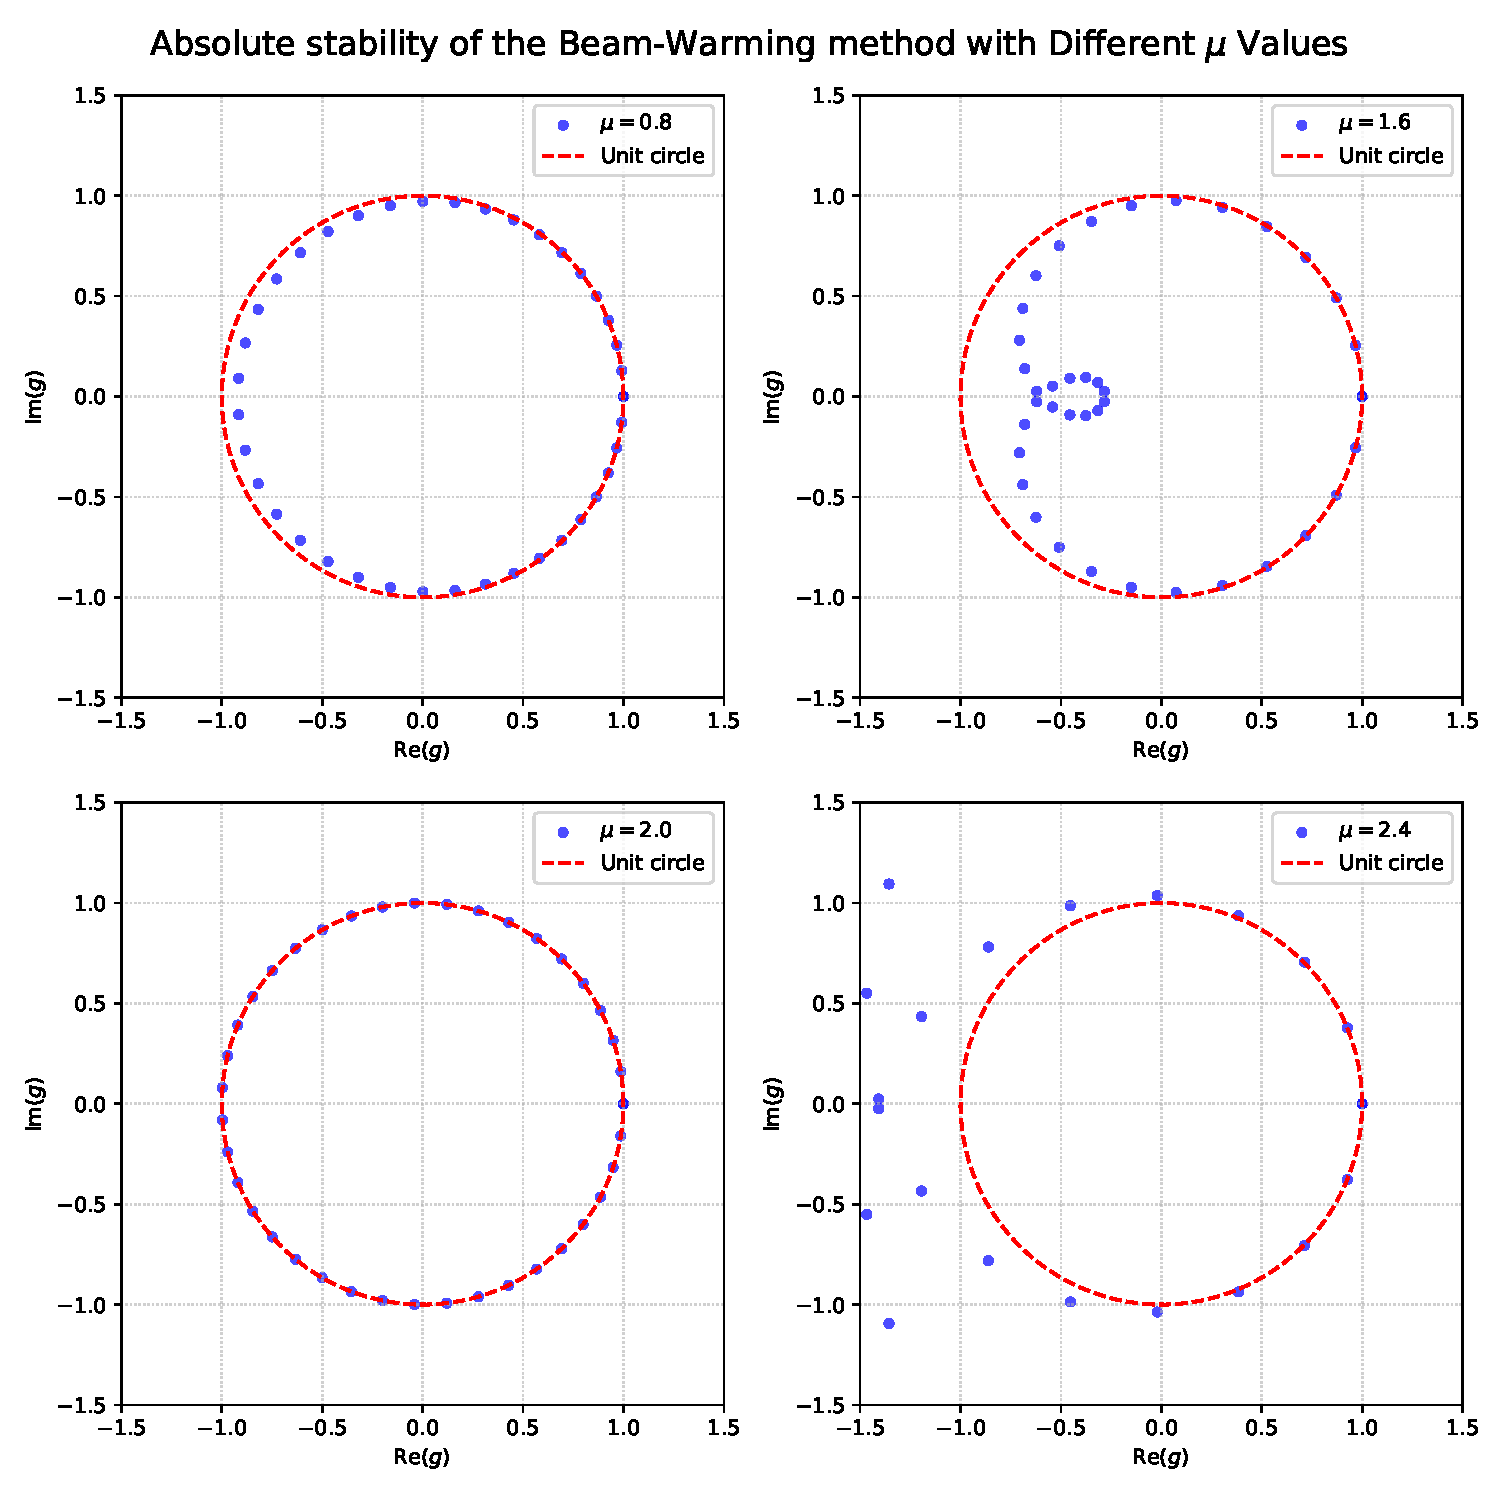
\includegraphics[width=0.6\textwidth]{figure/Exercise14.100.pdf}
    \caption{Exercise 14.100}
    \label{fig:Exercise14.100}
\end{figure}

\section*{Exercise 14.103}

\par upwind method 在 $a<0$ 时的离散格式为
\begin{equation}
    U_{j}^{n+1} = U_{j}^{n} - \mu\left(
        U_{j+1}^{n}-U_{j}^{n}    
        \right)
\end{equation}
\par 其数值依赖域如图 \ref{fig:Exercise14.103} 所示。
\begin{figure}[htbp]
    \centering
    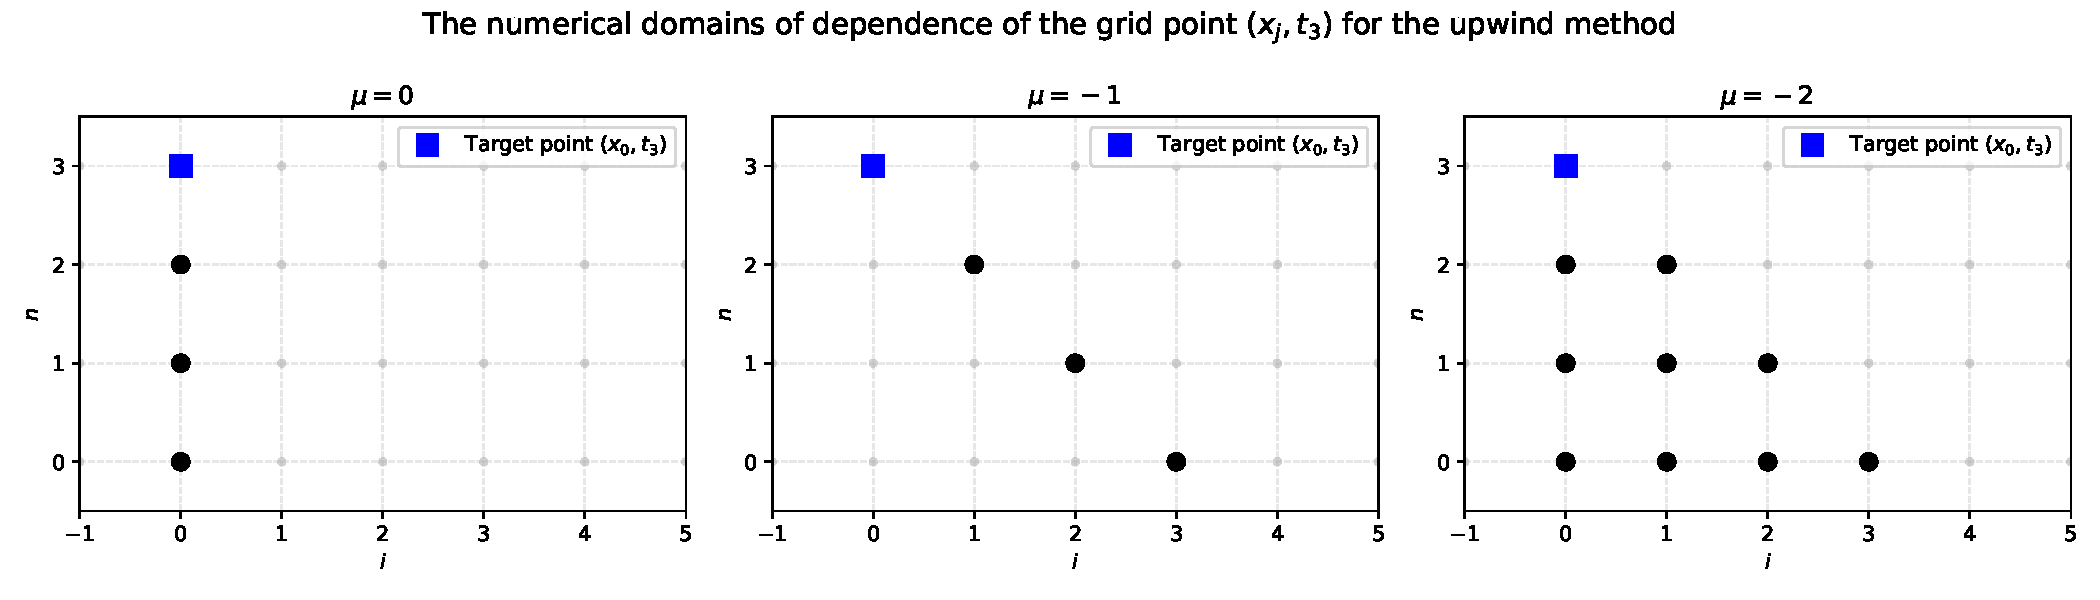
\includegraphics[width=\textwidth]{figure/Exercise14.103.pdf}
    \caption{Exercise 14.103}
    \label{fig:Exercise14.103}
\end{figure}

\section*{Exercise 14.104}

\par Lax-Wendrof method 的离散格式为
\begin{equation}
    U_{j}^{n+1} = U_{j}^{n} - \frac{\mu}{2}\left(
        U_{j+1}^{n}-U_{j-1}^{n}    
        \right)
        + \frac{\mu^2}{2}\left(
            U_{j+1}^{n}-2U_{j}^{n}+U_{j-1}^{n}
        \right)
\end{equation}
\par 其数值依赖域如图 \ref{fig:Exercise14.104} 所示。
\begin{figure}[htbp]
    \centering
    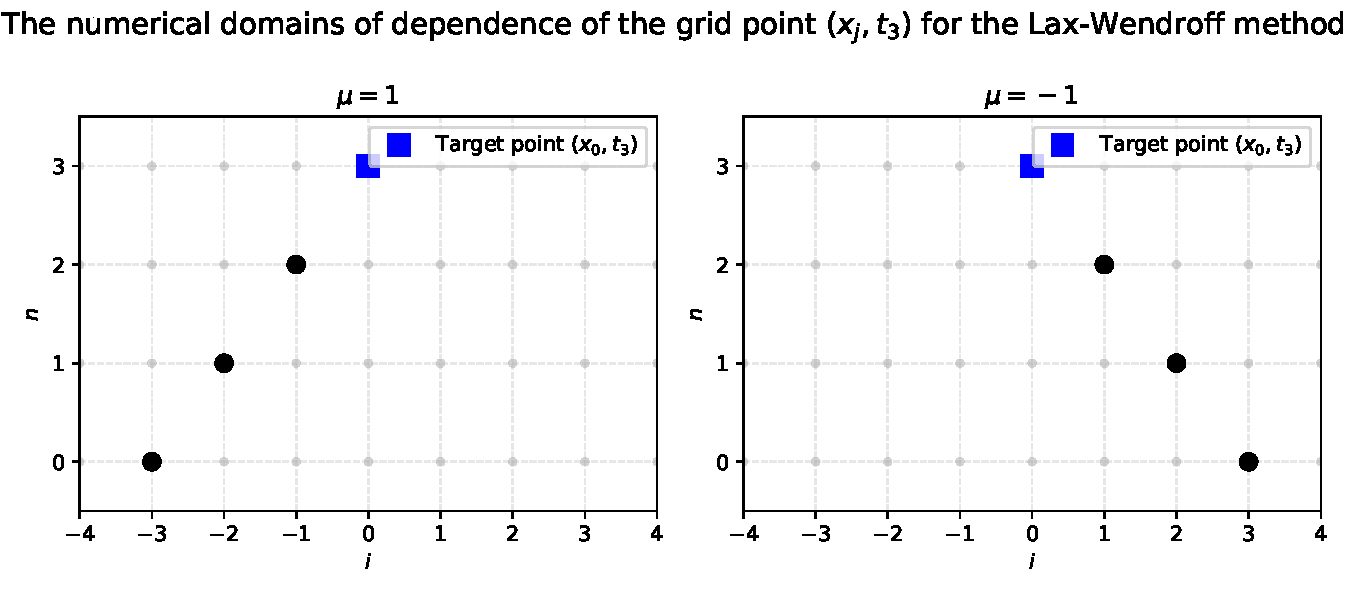
\includegraphics[width=0.67\textwidth]{figure/Exercise14.104.pdf}
    \caption{Exercise 14.104}
    \label{fig:Exercise14.104}
\end{figure}

\section*{Exercise 14.113}

\par leapfrog method 的离散格式为
\begin{equation}
    \frac{U_{j}^{n+1}-U_{j}^{n-1}}{2k} + a\frac{U_{j+1}^{n}-U_{j-1}^{n}}{2h} = 0
\end{equation}
\par 将 $U_{j}^{n}$ 用 $v(x_j, t_n)$ 代换
\begin{equation}
    \begin{gathered}  
        \frac{v(x_j, t_{n+1})-v(x_j, t_{n-1})}{2k} + a\frac{v(x_{j+1}, t_n)-v(x_{j-1}, t_n)}{2h}=0\\
        \frac{1}{2k}\left[
            \left(v+kv_t+\frac{1}{2}k^2v_{tt}+\frac{1}{6}k^3v_{ttt}\right)
            -\left(v-kv_t+\frac{1}{2}k^2v_{tt}-\frac{1}{6}k^3v_{ttt}\right)
            +O(k^4)
        \right]\qquad\qquad\qquad\\
        \qquad\qquad\qquad+\frac{a}{2h}\left[
            \left(v+hv_x+\frac{1}{2}h^2v_{xx}+\frac{1}{6}h^3v_{xxx}\right)
            -\left(v-hv_x+\frac{1}{2}h^2v_{xx}-\frac{1}{6}h^3v_{xxx}\right)
            +O(h^4)
        \right]=0\\
        v_t + av_x = -\frac{1}{6}k^2v_{ttt}-\frac{1}{6}ah^2v_{xxx}+O(k^3+h^3)
    \end{gathered}
\end{equation}
\par 对于 $v_{ttt}$，需要用 $v_{xxx}$ 来代替。由上式求导可得
\begin{equation}
    \begin{cases}
        v_{tt}
        = -av_{xt} + O(k^3+h^3)\\
        v_{xt}
        = -av_{xx} + O(k^3+h^3)\\
        v_{ttt}
        = -av_{xtt} + O(k^3+h^3)\\
        v_{xtt}
        = -av_{xxt} + O(k^3+h^3)\\
        v_{xxt}
        = -av_{xxx} + O(k^3+h^3)
    \end{cases}
\end{equation}
\par 综上 $v_{ttt} = -a^3v_{xxx} + O(k^2+h^2)$，所以
\begin{equation}
    \begin{gathered}
        v_t + av_x = \frac{1}{6}k^2a^3v_{xxx}-\frac{1}{6}ah^2v_{xxx}+O(k^3+h^3)\\
        v_t + av_x = \frac{1}{6}ah^2(\mu^2-1)v_{xxx}+O(k^3+h^3)
    \end{gathered}
\end{equation}
\par 如果考虑更高阶的情况，保留到第五项
\begin{equation}
    \begin{gathered}  
        \frac{v(x_j, t_{n+1})-v(x_j, t_{n-1})}{2k} + a\frac{v(x_{j+1}, t_n)-v(x_{j-1}, t_n)}{2h}=0\\
        v_t + av_x = 
        \left(-\frac{1}{6}k^2v_{ttt}-\frac{1}{6}ah^2v_{xxx}\right)
        +\left(-\frac{1}{120}k^4v_{ttttt}-\frac{1}{120}ah^4v_{xxxxx}\right)
        +O(k^5+h^5)
    \end{gathered}
\end{equation}
\par 最后得到
\begin{equation}
    v_t + av_x = \frac{1}{6}ah^2(\mu^2-1)v_{xxx} + \epsilon_f v_{xxxxx}
\end{equation}
\par 对于 Lax-Wendroff method，同样的计算可以得到
\begin{equation}
    \begin{gathered}  
        \frac{v(x_j,t_{n+1})-v(x_j,t_{n})}{k}
        +\frac{a}{2h}\left[
            v(x_{j+1},t_{n})-v(x_{j-1},t_{n})
        \right]=
        \frac{a^2k}{2h^2}\left[
            v(x_{j+1},t_{n})-2v(x_{j},t_{n})+v(x_{j-1},t_{n})
        \right]\\
        v_t+\frac{1}{2}kv_{tt} + \frac{1}{6}k^2v_{ttt}
        +av_x+\frac{ah^2}{6}v_{xxx}
        =\frac{k}{2}a^2v_{xx}
        +\frac{kh^2}{24}a^2v_{xxxx}+ O(h^3)\\
    \end{gathered}
\end{equation}
\par 最终可以得到
\begin{equation}
    v_t + av_x = \frac{1}{6}ah^2(\mu^2-1)v_{xxx} + \epsilon_w v_{xxxx}
\end{equation}

\section*{Exercise 14.114}
    
\par Beam-Warming method 在$a\geq 0$ 时的离散格式为
\begin{equation}
    U_{j}^{n+1} = U_{j}^{n} - \frac{\mu}{2}
        \left(
            3U_{j}^{n}-4U_{j-1}^{n}+U_{j-2}^{n}
        \right) + \frac{\mu^2}{2}
        \left(
            U_{j}^{n}-2U_{j-1}^{n}+U_{j-2}^{n}
        \right)
\end{equation}
\par 将 $U_{j}^{n}$ 用 $v(x_j, t_n)$ 代换
\begin{equation}
    \begin{gathered}
        \frac{v(x_j, t_{n+1})-v(x_j, t_{n})}{k} + \frac{a}{2h}\left[
            3v(x_j, t_n)-4v(x_{j-1}, t_n)+v(x_{j-2}, t_n)
        \right]\\
        -\frac{a^2k}{2h^2}\left[
            v(x_j, t_n)-2v(x_{j-1}, t_n)+v(x_{j-2}, t_n)
        \right]=0\\
        \frac{1}{k}\left[
            \left(v+kv_t+\frac{1}{2}k^2v_{tt}+\frac{1}{6}k^3v_{ttt}\right)
            -v
            +O(k^4)
        \right]\qquad\qquad\qquad\qquad\qquad\qquad\qquad\qquad\qquad\qquad\qquad\\
        +\frac{a}{2h}\left[
            3v-4\left(v-hv_x+\frac{1}{2}h^2v_{xx}-\frac{1}{6}h^3v_{xxx}\right)
            +\left(v-2hv_x+\frac{1}{2}(2h)^2v_{xx}-\frac{1}{6}(2h)^3v_{xxx}\right)
            +O(h^4)
        \right]\\
        \qquad-\frac{a^2k}{2h^2}\left[
            v-2\left(v-hv_x+\frac{1}{2}h^2v_{xx}-\frac{1}{6}h^3v_{xxx}\right)
            +\left(v-2hv_x+\frac{1}{2}(2h)^2v_{xx}-\frac{1}{6}(2h)^3v_{xxx}\right)
            +O(h^4)
        \right]=0\\
        v_t+\frac{1}{2}kv_{tt}+\frac{1}{6}k^2v_{ttt}
        +av_x-\frac{ah^2}{3}v_{xxx}
        -\frac{a^2k}{2}v_{xx}+\frac{a^2kh}{2}v_{xxx}+O(k^3+h^3)=0\\
        v_t + av_x 
        +\left(
            \frac{1}{2}kv_{tt} - \frac{a^2k}{2}v_{xx}
        \right)
        +\left(
            \frac{1}{6}k^2v_{ttt} - \frac{ah^2}{3}v_{xxx} + \frac{a^2kh}{2}v_{xxx}
        \right)
        = O(k^3+h^3)
    \end{gathered}
\end{equation}
\par 最后得到
\begin{equation}
    v_t + av_x = \frac{ah^2}{6}(2-3\mu+\mu^2)v_{xxx} + O(k^3+h^3)
\end{equation}
\par 从该式子可知 $w = a\xi + \dfrac{ah^2}{6}(\mu-1)(\mu-2)v_{xxx}\xi^3$，
从而得到
\begin{equation}
    \begin{gathered}
        C_p(\xi)= a + \dfrac{ah^2}{6}(\mu-1)(\mu-2)\xi^2\\
        C_g(\xi)= a + \dfrac{ah^2}{2}(\mu-1)(\mu-2)\xi^2
    \end{gathered}
\end{equation}
\par 可以看到两种均大于真实波速 $a$，
因此数值解中波纹出现在真实波峰的前方。

\section*{Exercise 14.115}

\par 当 $\mu=1$ 时，Lax-Wendroff 和 leapfrog method 的 modified equation 
中的 $v_{xxx}$ 项消失，低阶耗散消失。因此对于 $u_t+u_x=0$ 的数值模拟来说，
$k=h$ 时模拟的结果效果最好。

\section*{Program 14.4.1}

\begin{enumerate}
    \item[(a)] \textbf{Example 14.42} 结果的
    复现如图 \ref{fig:Exact_solution}
    至 \ref{fig:Collocation_RK_r_1} 所示。
    \begin{figure}[htbp]
        \centering
        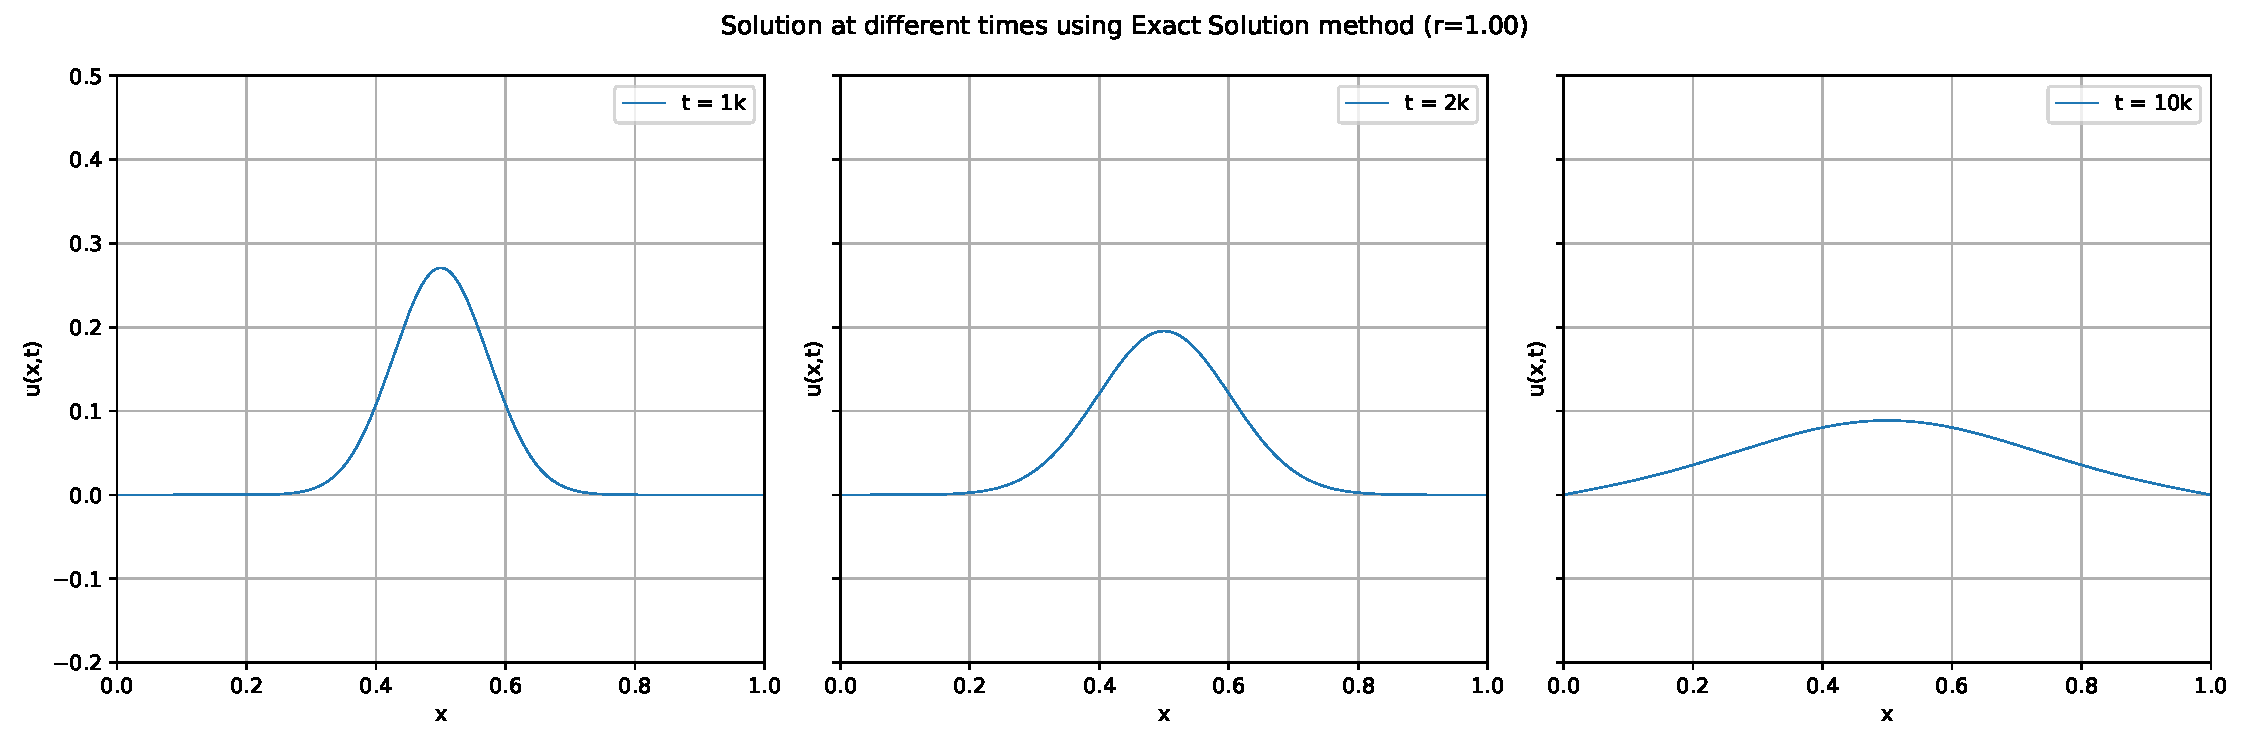
\includegraphics[width=1\textwidth]{figure/Exact_solution.pdf}
        \caption{Exact solution}
        \label{fig:Exact_solution}
    \end{figure}

    \begin{figure}[htbp]
        \centering
        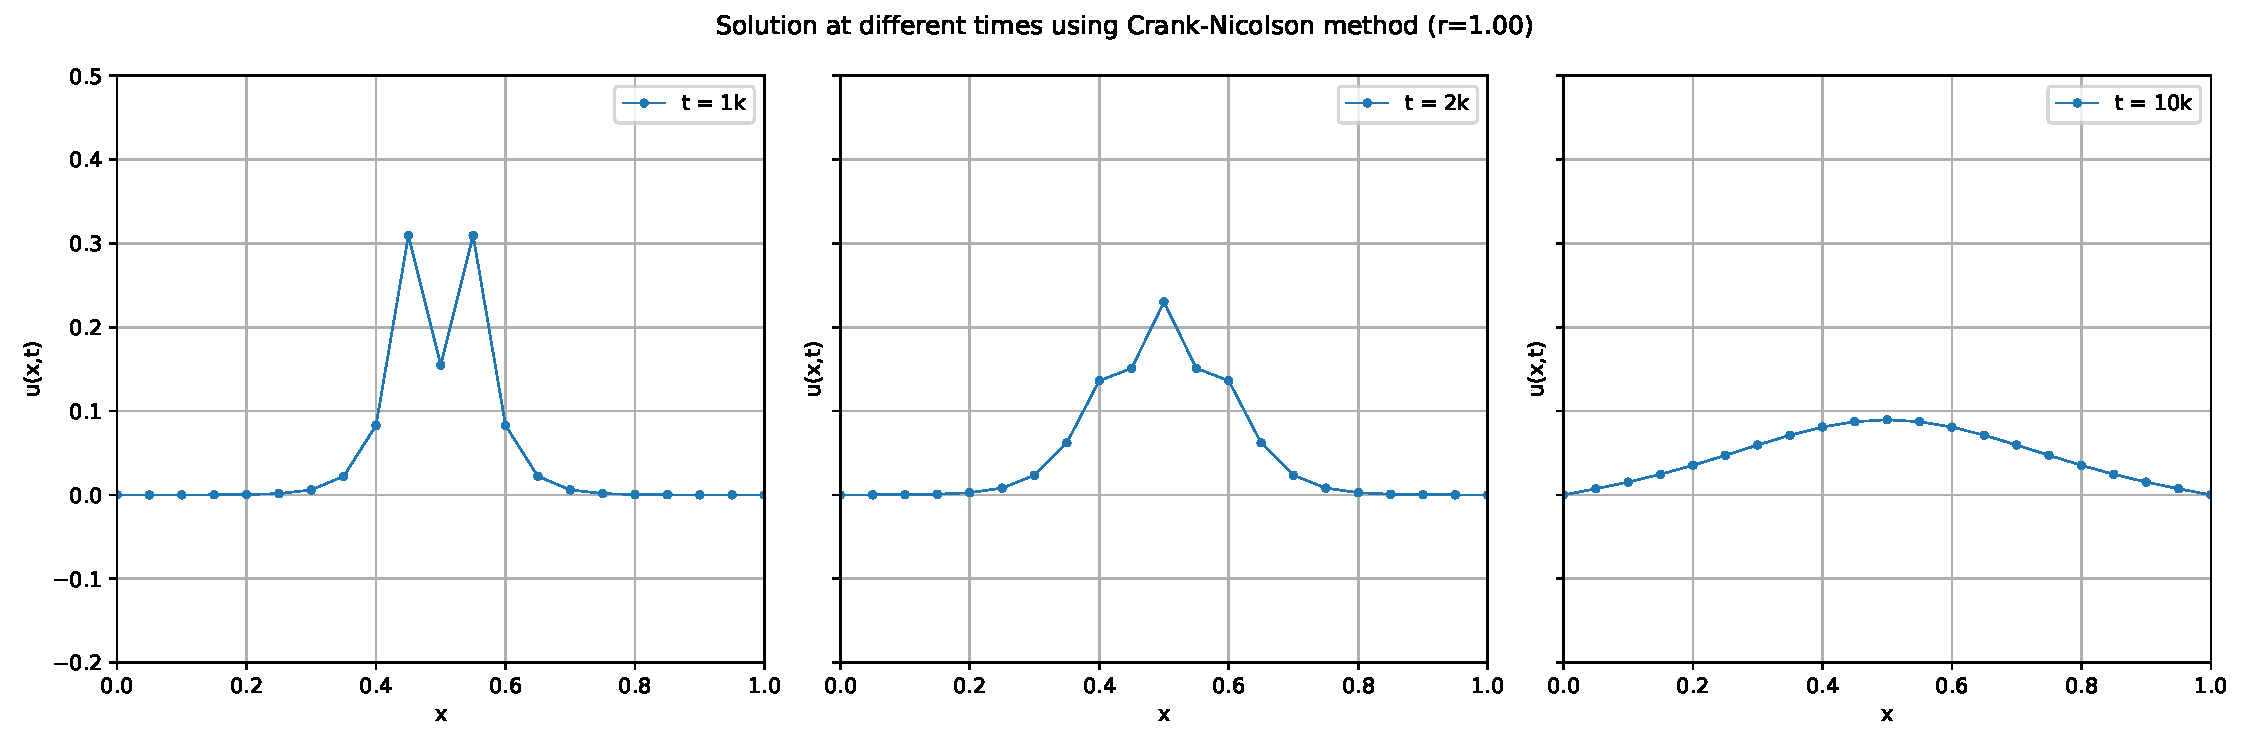
\includegraphics[width=1\textwidth]{figure/Crank-Nicolson_r_1.pdf}
        \caption{Crank-Nicolson method}
        \label{fig:Crank-Nicolson_r_1}
    \end{figure}

    \begin{figure}[htbp]
        \centering
        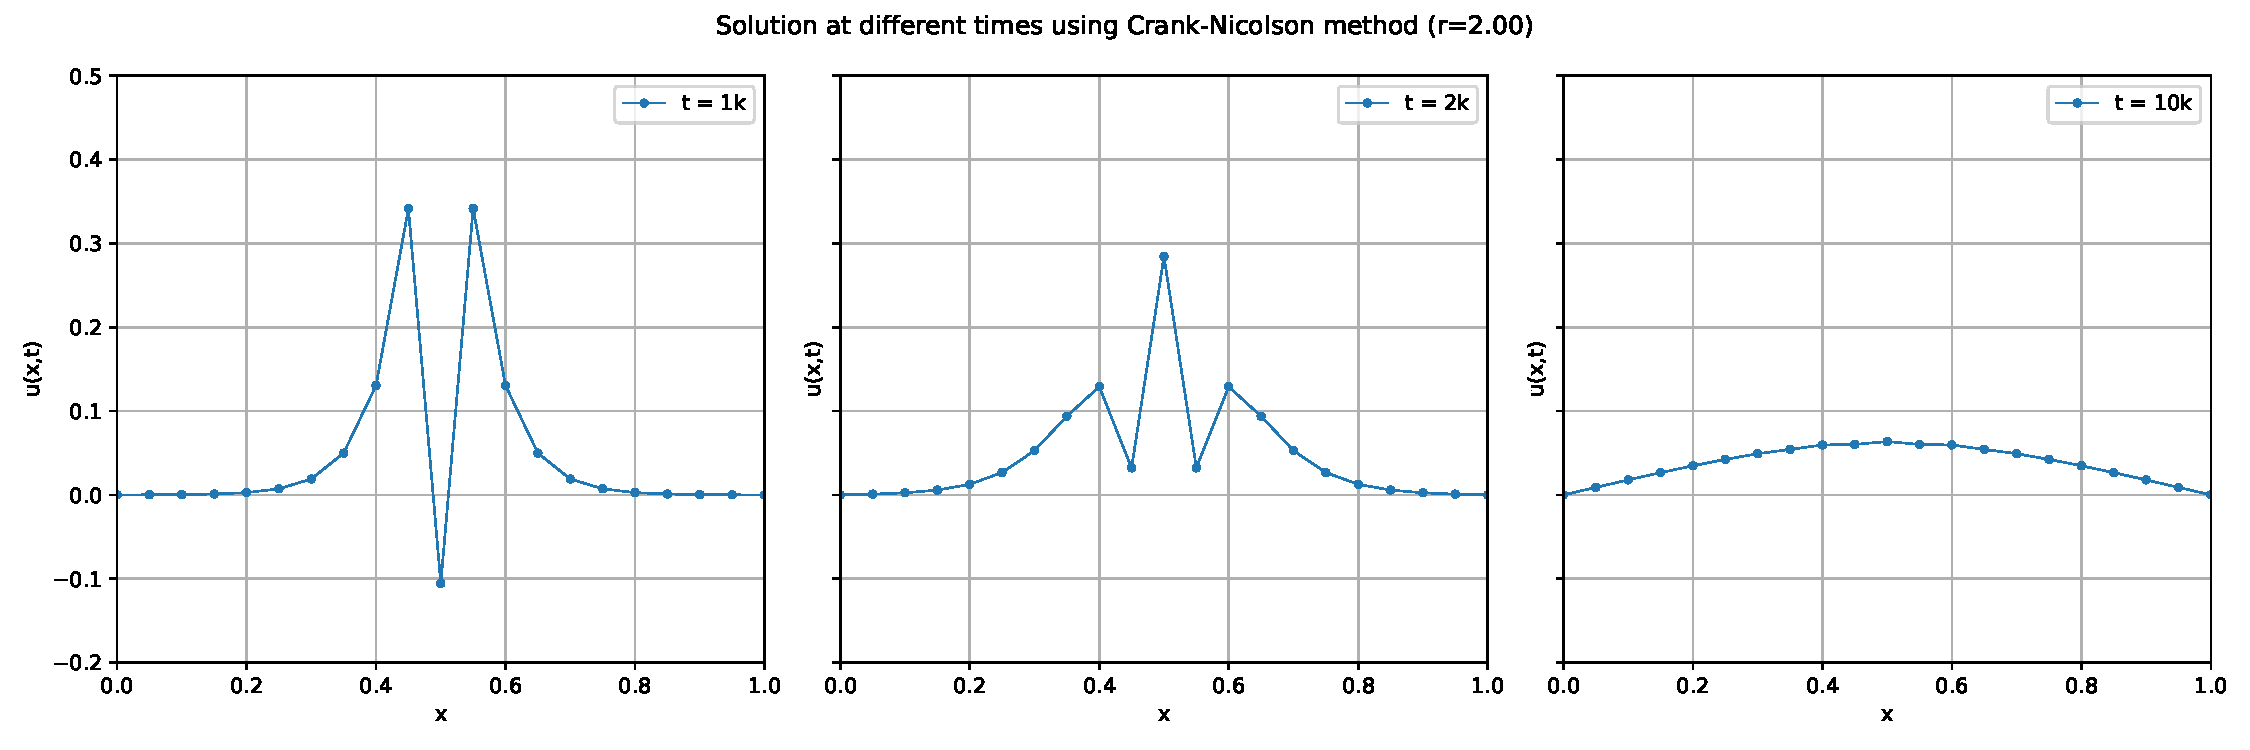
\includegraphics[width=1\textwidth]{figure/Crank-Nicolson_r_2.pdf}
        \caption{Crank-Nicolson method}
        \label{fig:Crank-Nicolson_r_2}
    \end{figure}

    \begin{figure}[htbp]
        \centering
        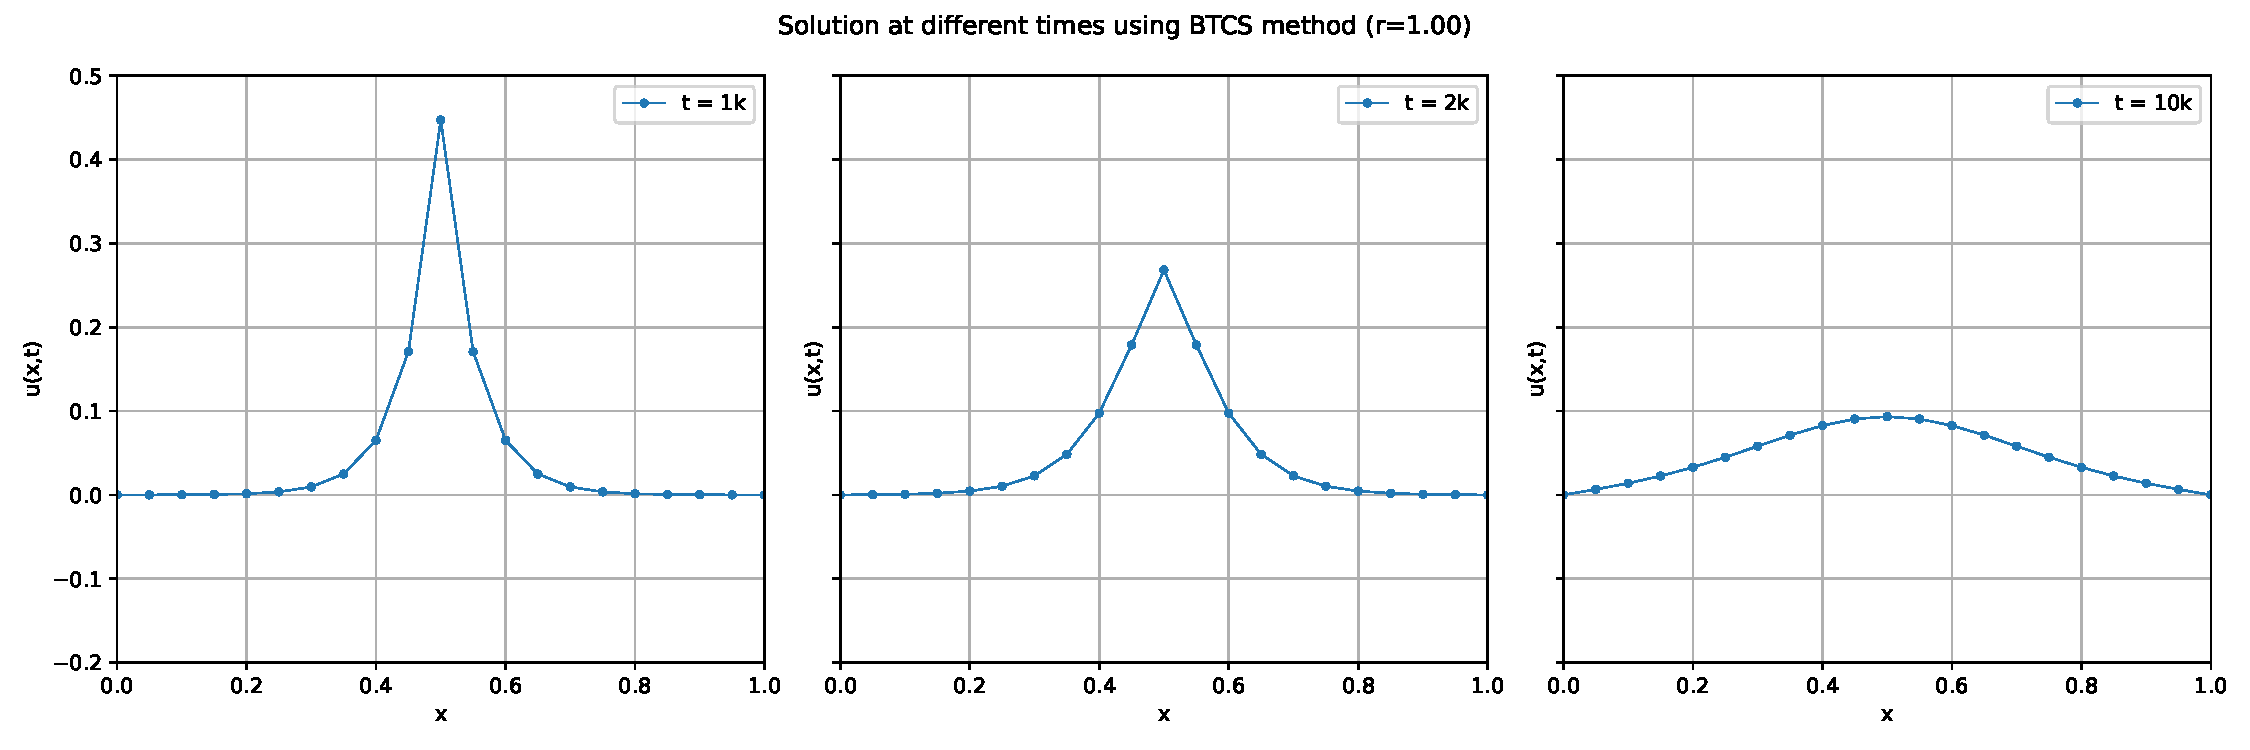
\includegraphics[width=1\textwidth]{figure/BTCS_r_1.pdf}
        \caption{BTCS method}
        \label{fig:BTCS_r_1}
    \end{figure}

    \begin{figure}[htbp]
        \centering
        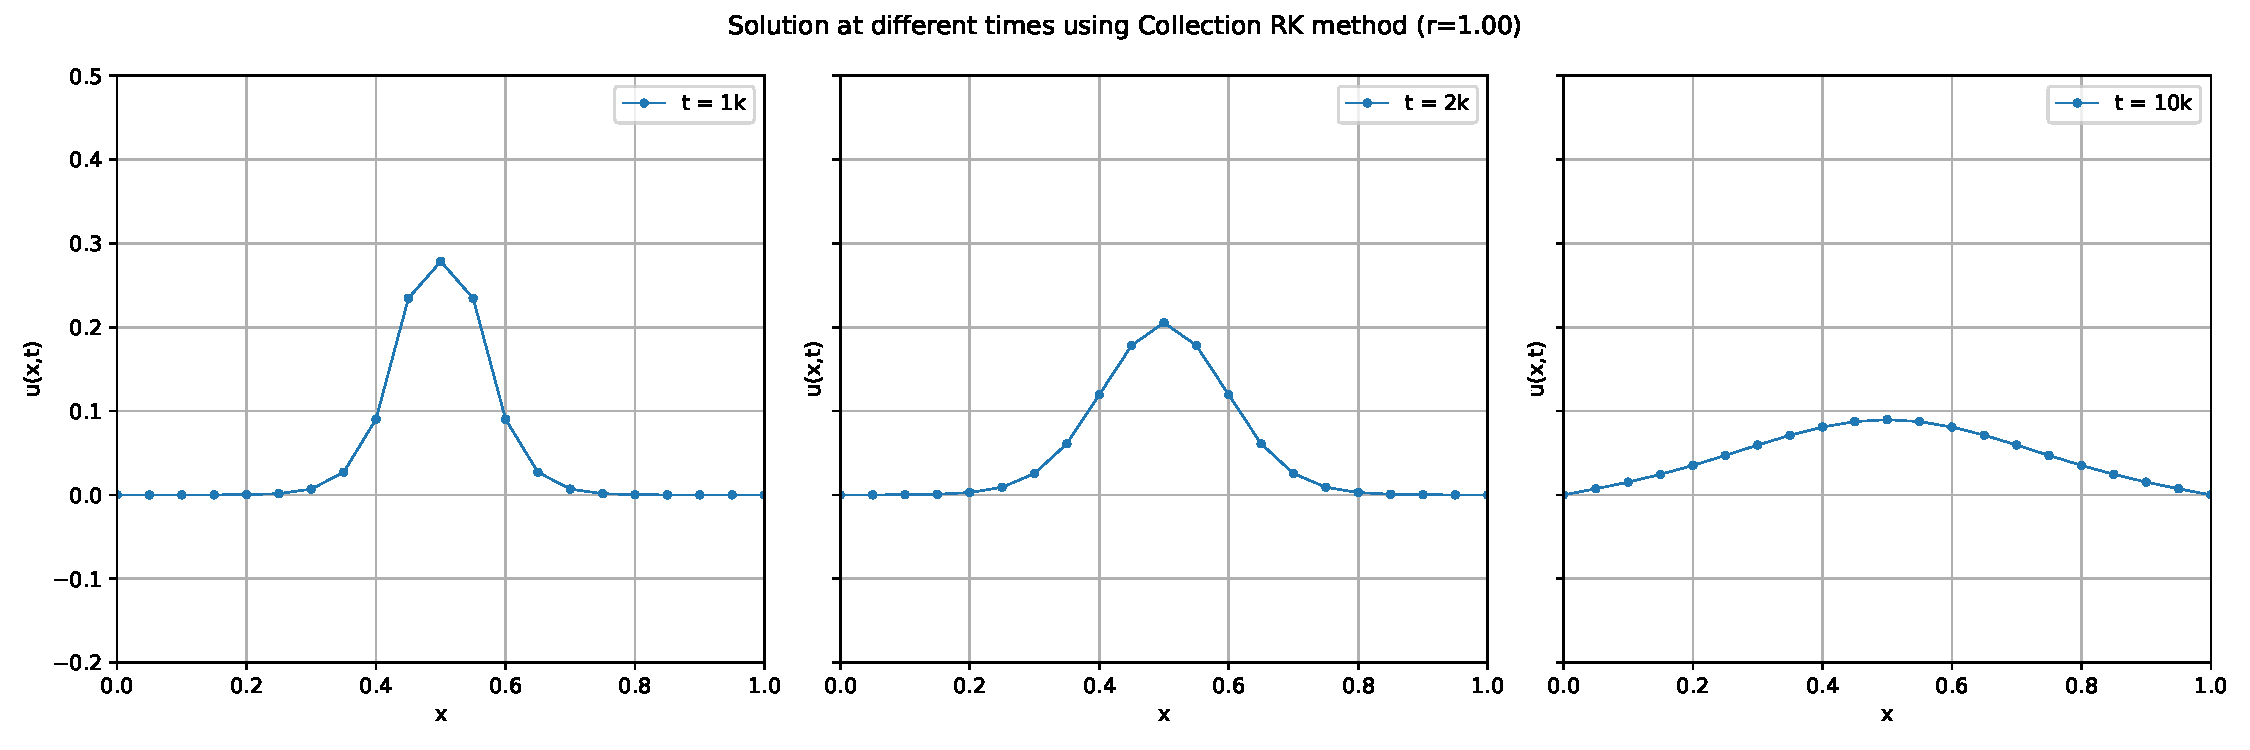
\includegraphics[width=1\textwidth]{figure/Collection_RK_r_1.pdf}
        \caption{Collocation method}
        \label{fig:Collocation_RK_r_1}
    \end{figure}
    \item[(b)] $r = \dfrac{1}{2h} = 10$ 时
    的 BTCS method 如图 \ref{fig:BTCS_r_10} 所示。
    \begin{figure}[htbp]
        \centering
        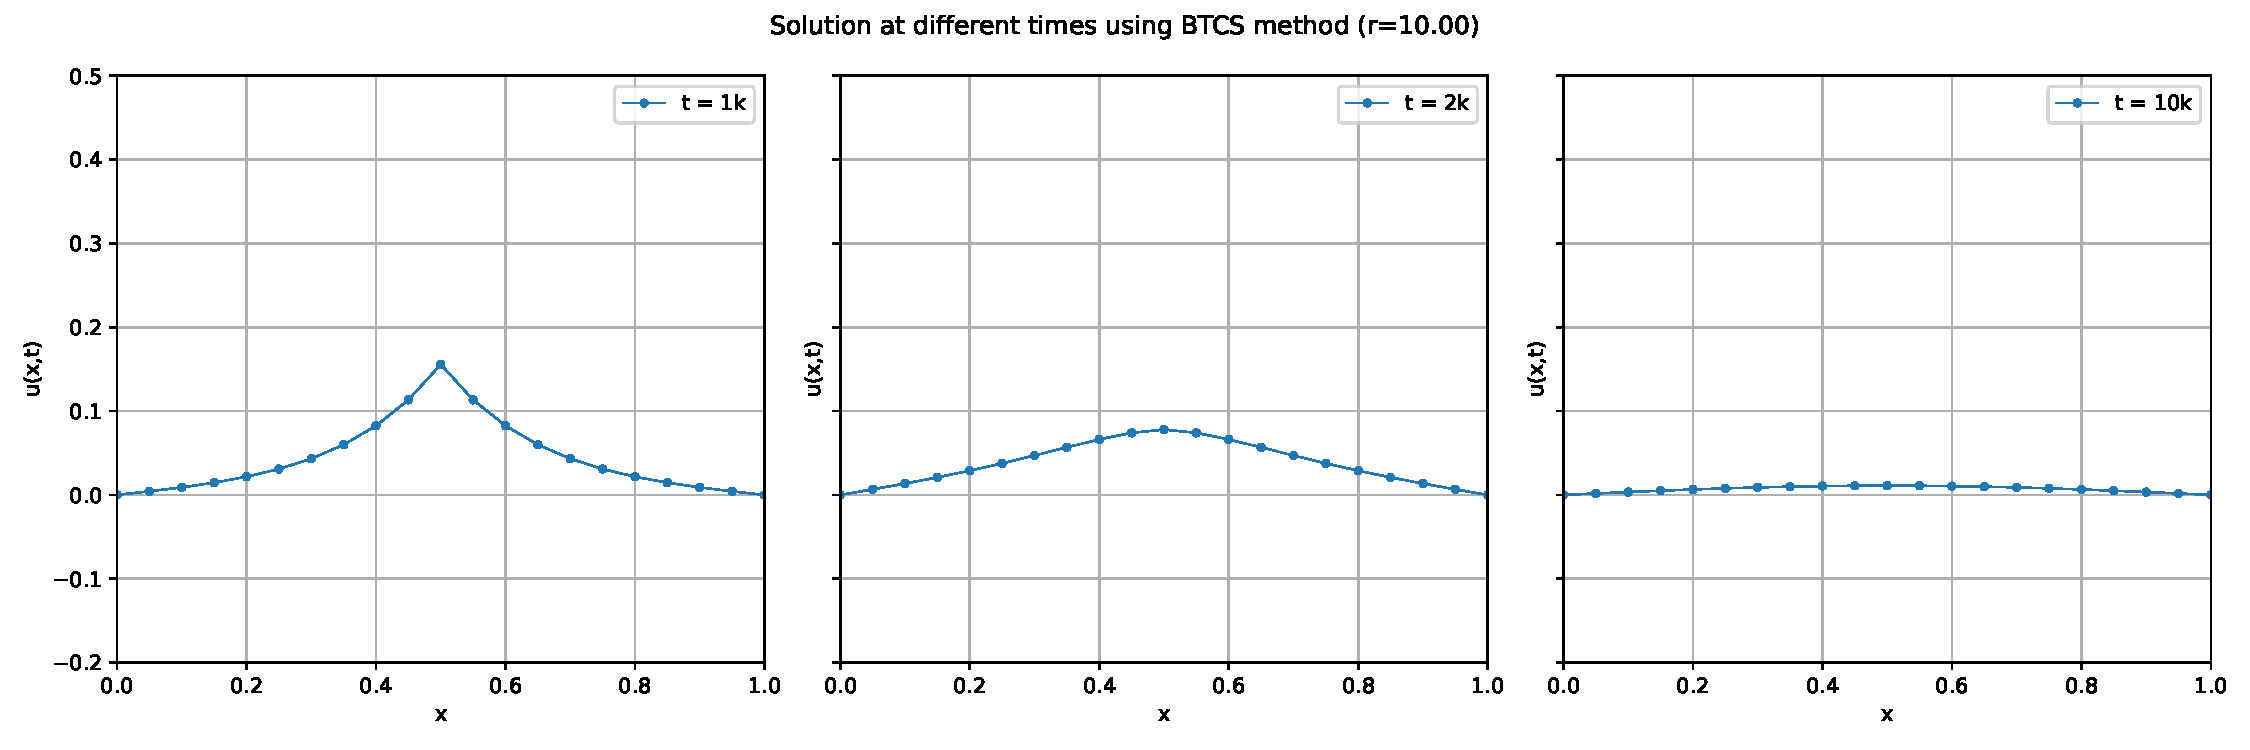
\includegraphics[width=1\textwidth]{figure/BTCS_r_10.pdf}
        \caption{BTCS method}
        \label{fig:BTCS_r_10}
    \end{figure}
    \item[(c)] $r = 0.5$ 和 $r = 1$ 时的 FTCS method 如图 \ref{fig:FTCS_r_0.5} 和 \ref{fig:FTCS_r_1} 所示。
    \begin{figure}[htbp]
        \centering
        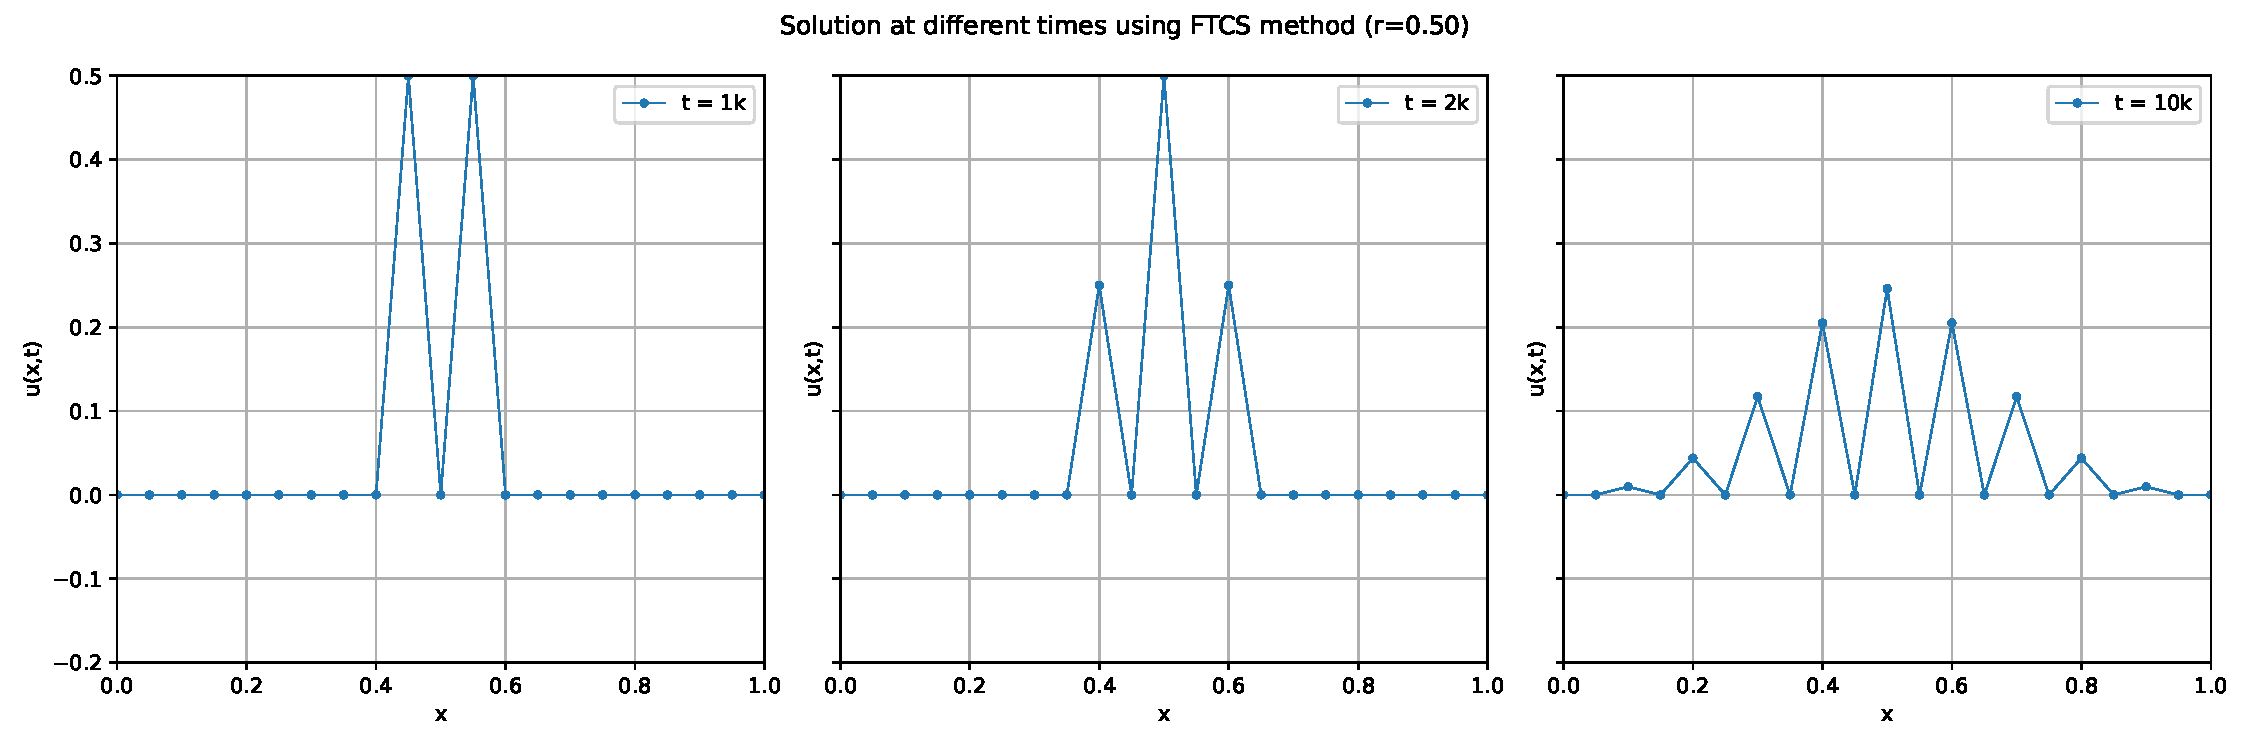
\includegraphics[width=1\textwidth]{figure/FTCS_r_0.5.pdf}
        \caption{FTCS method}
        \label{fig:FTCS_r_0.5}
    \end{figure}
    
    \begin{figure}[htbp]
        \centering
        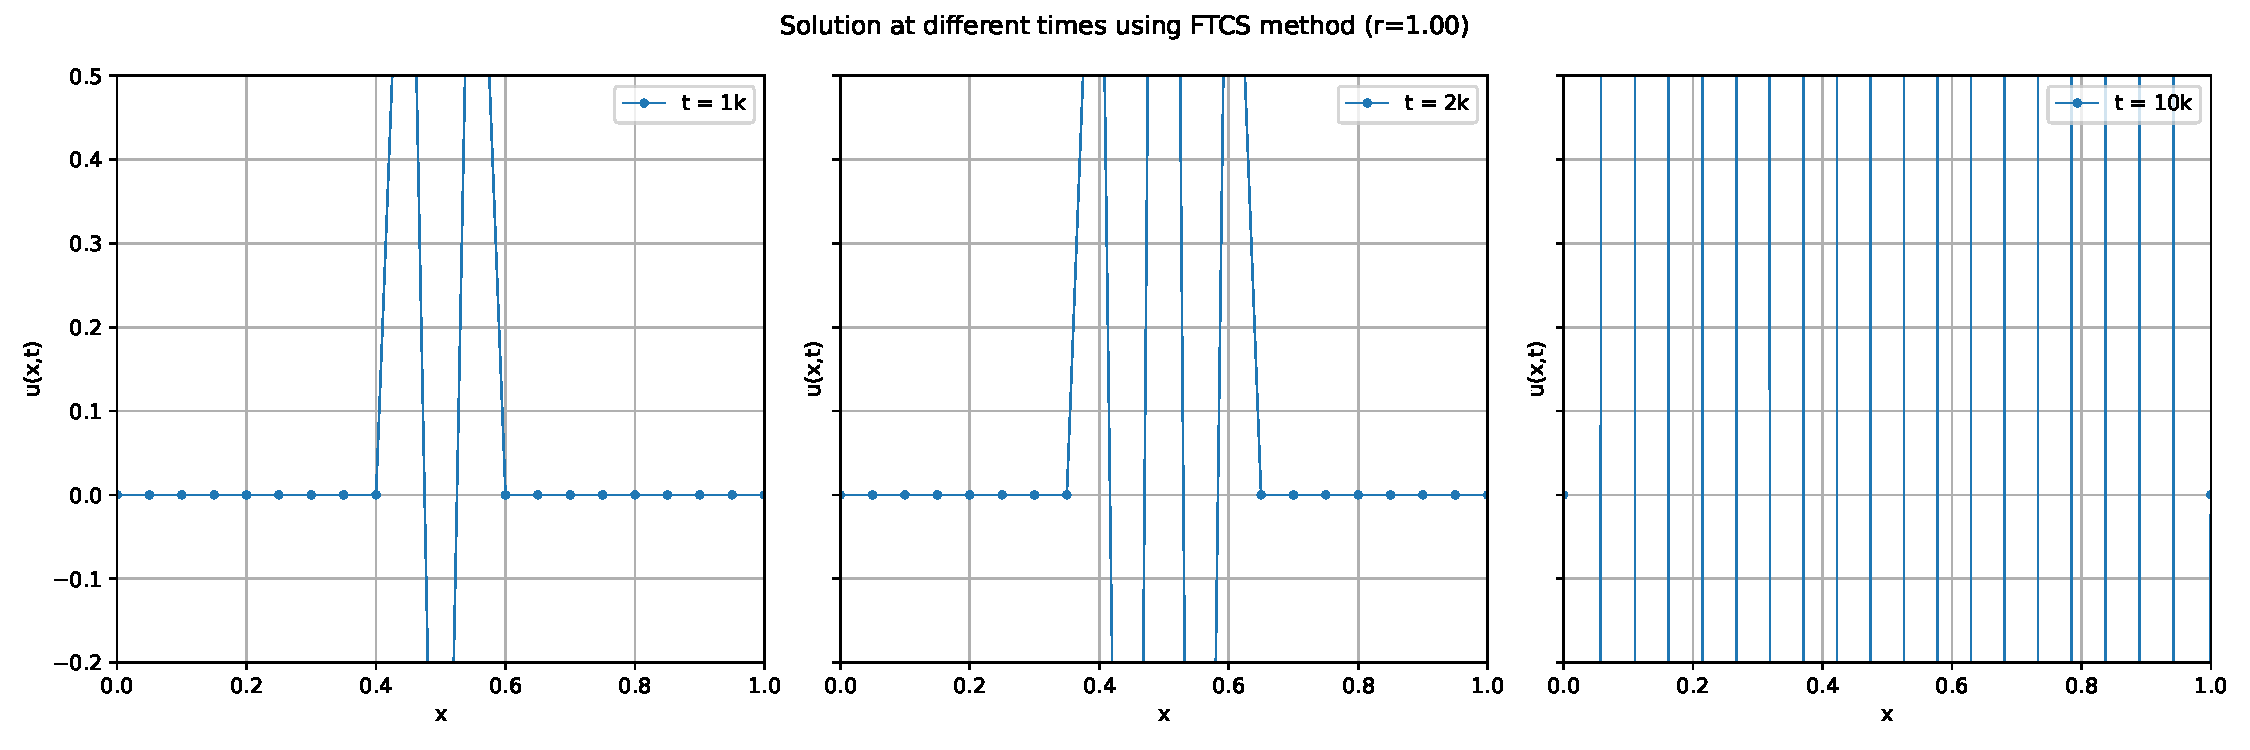
\includegraphics[width=1\textwidth]{figure/FTCS_r_1.pdf}
        \caption{FTCS method}
        \label{fig:FTCS_r_1}
    \end{figure}
    \item[(d)] $r = 1$ 和 $r = 10$ 时的 Gauss-Legendre RK method 如图 \ref{fig:Gauss-Legendre_RK_r_1} 和 \ref{fig:Gauss-Legendre_RK_r_10} 所示。
    \begin{figure}[htbp]
        \centering
        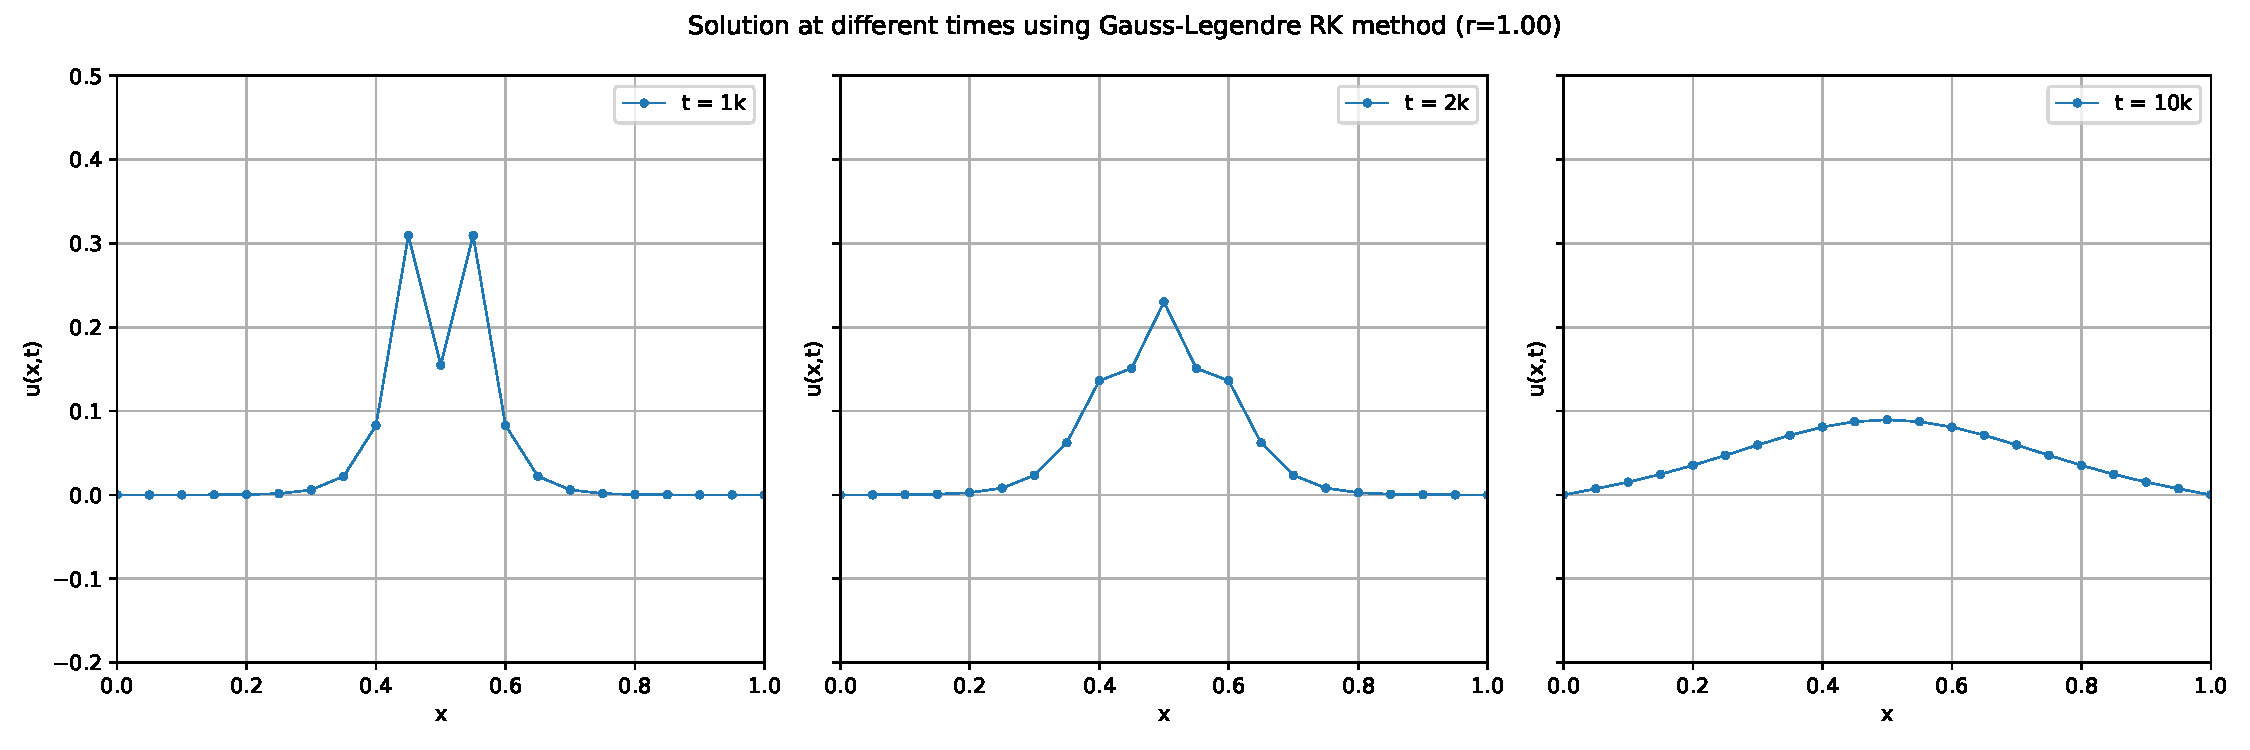
\includegraphics[width=1\textwidth]{figure/Gauss-Legendre_RK_r_1.pdf}
        \caption{Gauss-Legendre RK method}
        \label{fig:Gauss-Legendre_RK_r_1}
    \end{figure}

    \begin{figure}[htbp]
        \centering
        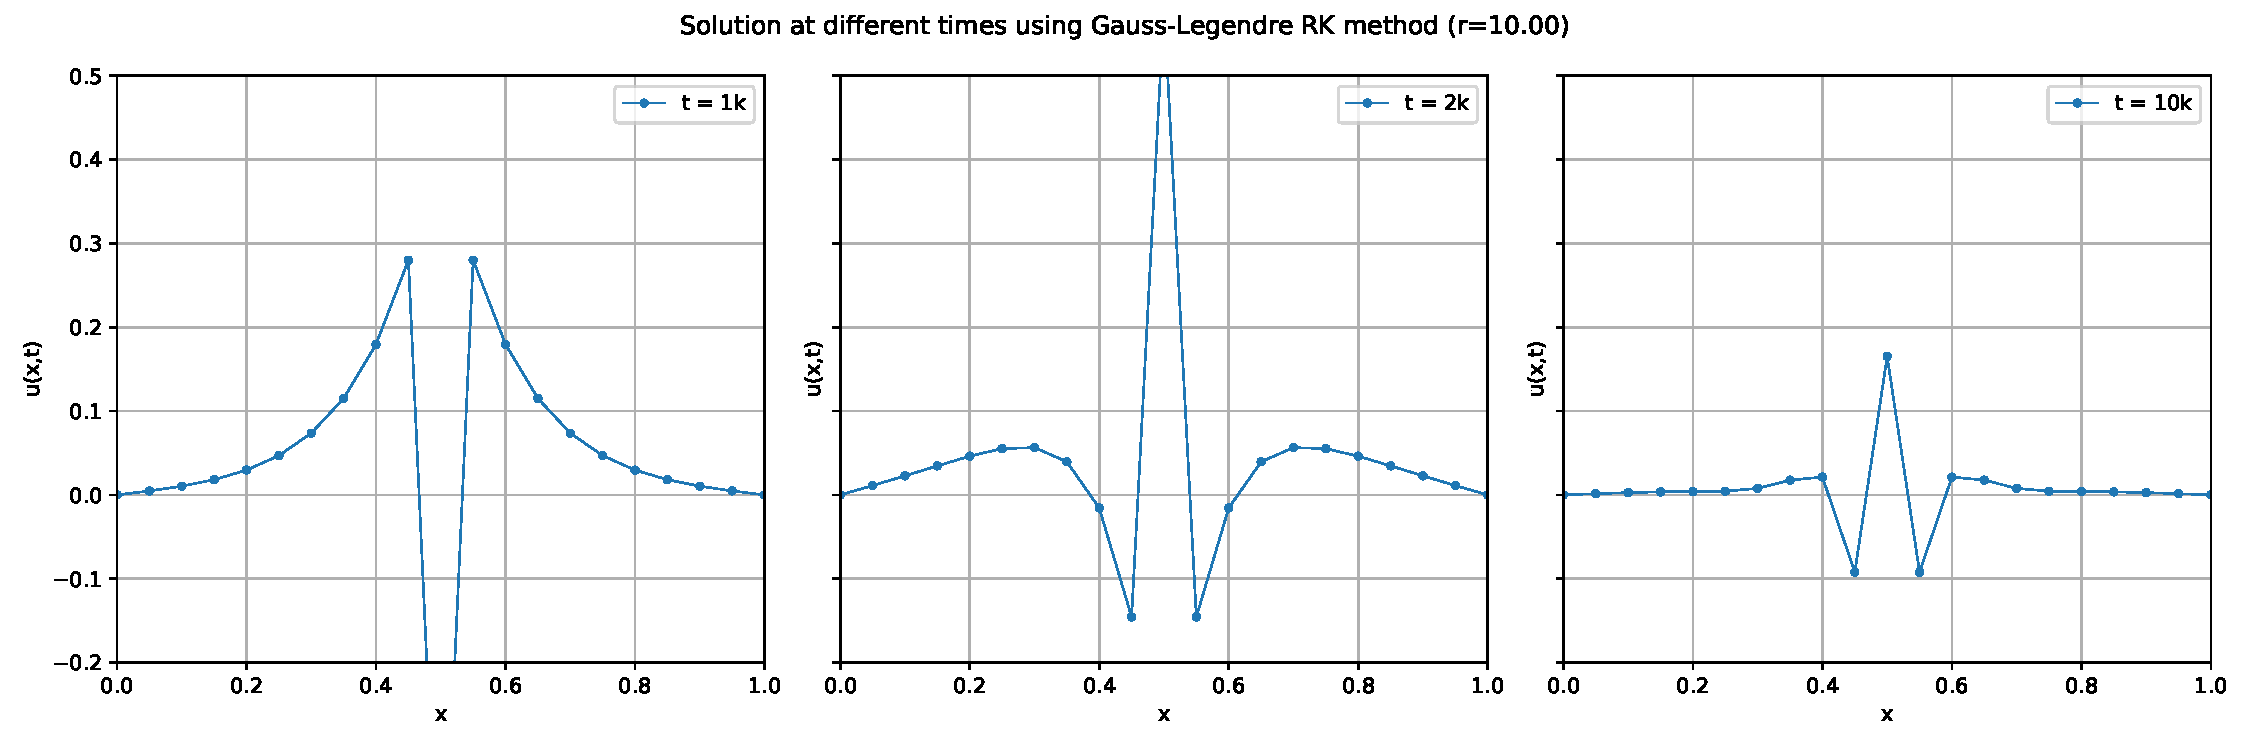
\includegraphics[width=1\textwidth]{figure/Gauss-Legendre_RK_r_10.pdf}
        \caption{Gauss-Legendre RK method}
        \label{fig:Gauss-Legendre_RK_r_10}
    \end{figure}
    \item[(e)] 观察到的结论包括
    \begin{enumerate}
        \item [(i)] 大部分方法在 $t=10k$ 时的数值解
        相较于起始状态都比较接近精确解；
        \item [(ii)] Crank-Nicolson method 和 Gauss-Legendre RK method 两种数值方法
        得到结果非常近似，实际上他们是等价的；
        \item [(iii)] FTCS method 在 $r=1$ 时的数值解出现了明显的振荡，该显示方法
        在 $r=0.5$ 和 $r=1$ 时不稳定；
        \item [(iv)] 大部分方法在 $r=10$ 时的数值解都不能很好地逼近精确解，
        这是由于时间$k$相对于空间$h$太大导致的。
    \end{enumerate}
\end{enumerate}

\section*{Program 14.4.2}

\par \textbf{Example 14.108} 结果的
复现如图 \ref{fig:leapfrog_method}
至 \ref{fig:upwind_method} 所示。

\begin{enumerate}
    \item[(a)] 因为 Lax-Friedrichs method 和 upwind method 都是一阶精度方法，
    因此误差中低频分量明显，压制了高频分量；而剩下的三种方法都是二阶精度方法，所以会抖动更加明显。
    \item[(b)] 是由于色散误差导致的，
    初始解中包含一个陡峭的窄gaussian脉冲，数值解中
    不同频率的波以不同的速度传播，导致数值解中出现了波纹。
    \item[(c)] 计算两种方法的 $|g(h\xi)|$
    \par leapfrog method 的计算如下
    \begin{equation}
        \begin{gathered}
            U_{j}^{n+1} = U_{j}^{n-1} - \mu\left(
                U_{j+1}^{n} - U_{j-1}^{n}
            \right)\\
            g-g^{-1} = -\mu\left(
                e^{\mathbf{i}h\xi}-e^{-\mathbf{i}h\xi}
            \right)\\
            g^2 + 2\mathbf{i}\mu\sin(h\xi)g - 1 = 0\\
            g = -\mathbf{i}\mu\sin(h\xi) \pm \sqrt{1-\mu^2\sin^2(h\xi)}\\
            |g| = 1
        \end{gathered}
    \end{equation}
    \par Lax-Wendroff method 的计算如下
    \begin{equation}
        \begin{gathered}
            U_{j}^{n+1} = U_{j}^{n} - \frac{\mu}{2}\left(
                U_{j+1}^{n}-U_{j-1}^{n}    
                \right)
                + \frac{\mu^2}{2}\left(
                    U_{j+1}^{n}-2U_{j}^{n}+U_{j-1}^{n}
                \right)\\
            g = 1 - \frac{\mu}{2}\left(
                e^{\mathbf{i}h\xi}-e^{-\mathbf{i}h\xi}    
                \right)
                + \frac{\mu^2}{2}\left(
                    e^{\mathbf{i}h\xi}-2+e^{-\mathbf{i}h\xi}    
                \right)\\
            g = 1 - \mathbf{i}\mu\sin(h\xi)
                + \mu^2\left(
                    \cos(h\xi)-1
                \right)\\
            |g|^2 =
            1-\mu^2(1-\mu^2)\left(
                \cos(h\xi)-1
            \right)^2\leq 1
        \end{gathered}
    \end{equation}
    \par 由于 Lax-Wendroff method 的 $|g|$ 小于 1，因此数值解中波纹的振幅会逐渐减小，而 leapfrog method 的 $|g|$ 等于 1，因此数值解中波纹的振幅不会减小。
    导致后者的数值解中波纹更加明显。
    \item[(d)] 在 \text{Exercise 14.113} 中得到，对于 Lax-Wendroff method 
    的 modified equation 为
    \begin{equation}
        v_t + av_x +\frac{1}{6}ah^2(1-\mu^2)v_{xxx}=0
    \end{equation}
    \par 从该式子可知 $w = a\xi + \dfrac{ah^2}{6}(\mu^2-1)v_{xxx}\xi^3$，
    从而得到
    \begin{equation}
        \begin{gathered}
            C_p(\xi)= a + \dfrac{ah^2}{6}(\mu^2-1)\xi^2\\
            C_g(\xi)= a + \dfrac{ah^2}{2}(\mu^2-1)\xi^2
        \end{gathered}
    \end{equation}
    \par 当 $k=0.8h$也就是 $\mu=0.8$ 时，可以看到两种均小于真实波速 $a$，
    因此数值解中波纹出现在真实波峰的后方。
    \item[(e)] 在 \text{Exercise 14.114} 中已经回答。
    \item[(f)] 在 \text{Exercise 14.115} 中已经回答。
\end{enumerate}

\begin{figure}[htbp]
    \centering
    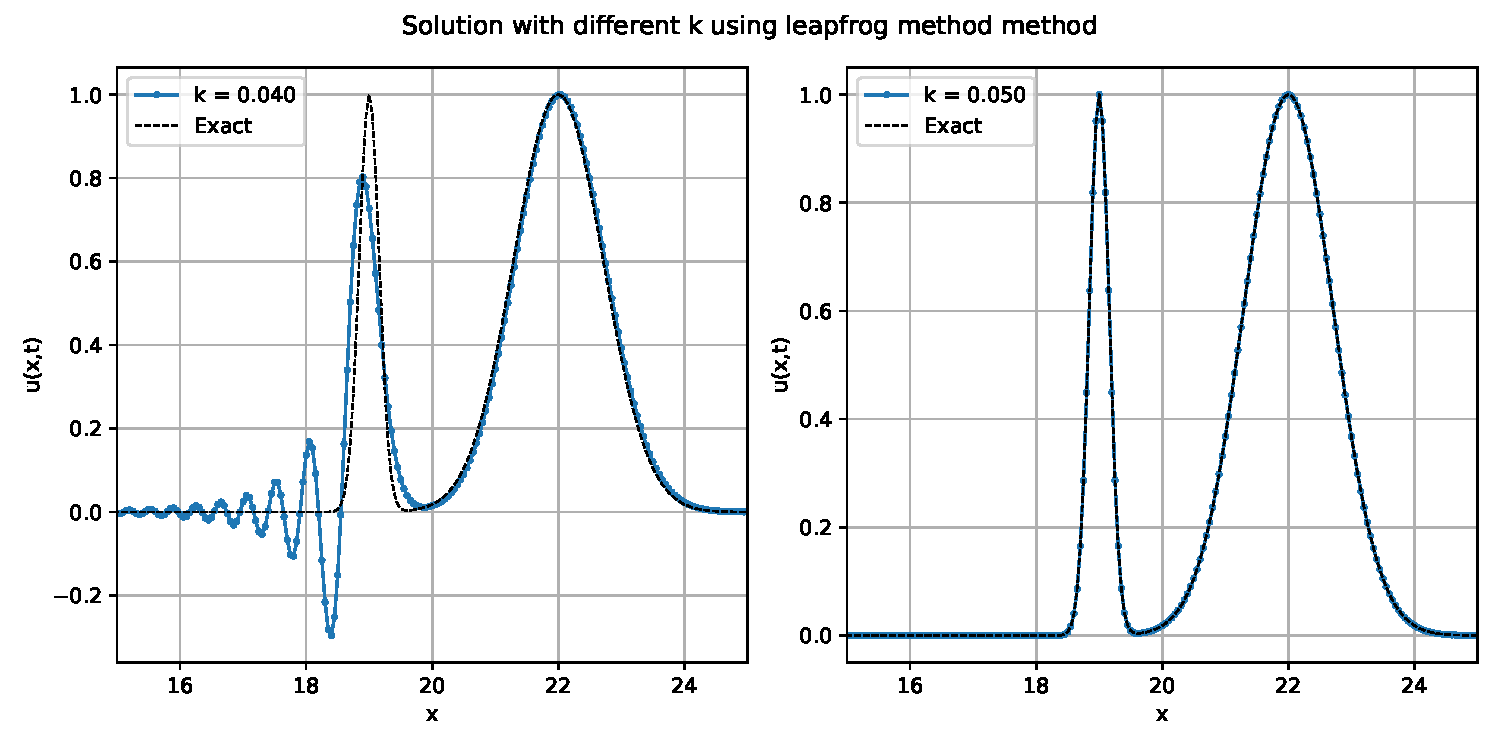
\includegraphics[width=0.67\textwidth]{figure/leapfrog_method.pdf}
    \caption{leapfrog method}
    \label{fig:leapfrog_method}
\end{figure}

\begin{figure}[htbp]
    \centering
    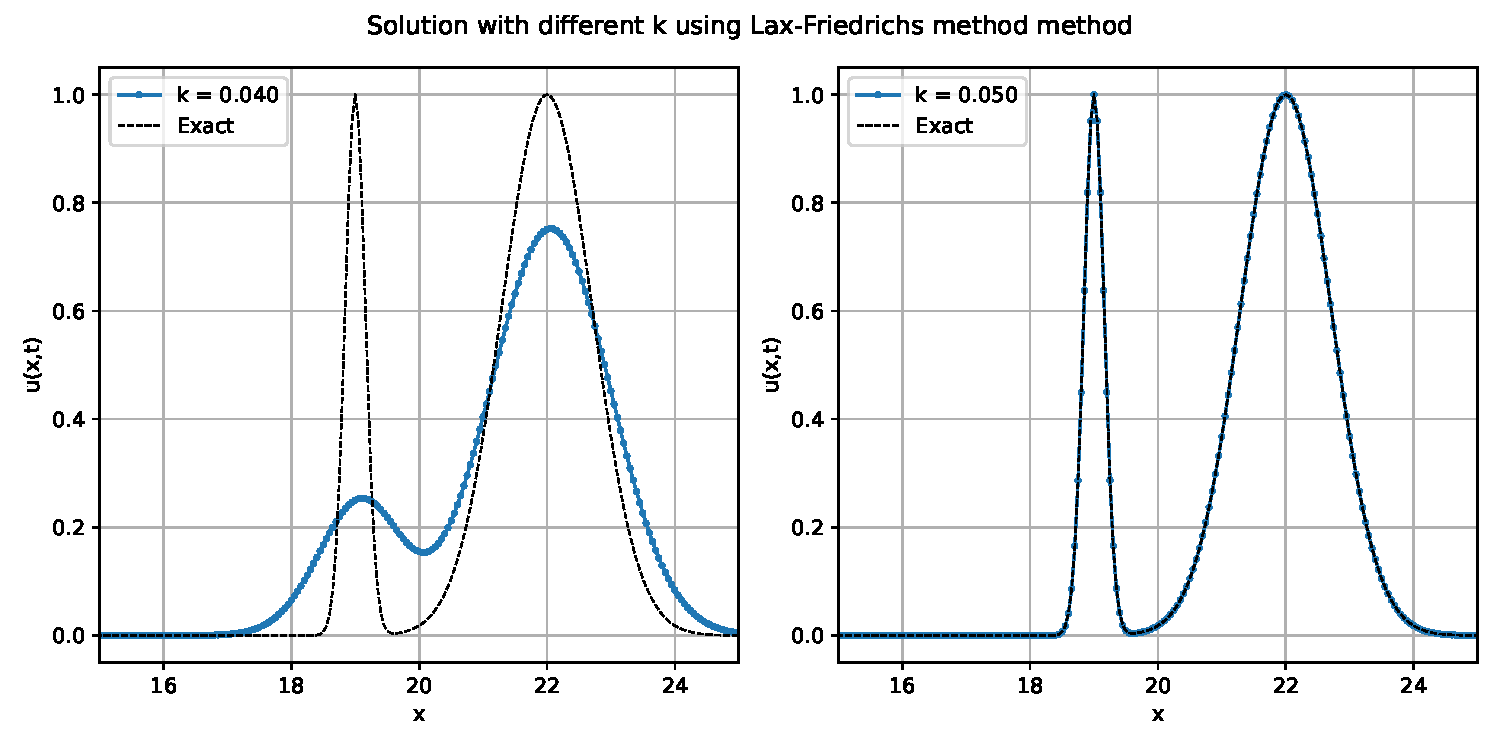
\includegraphics[width=0.67\textwidth]{figure/Lax-Friedrichs_method.pdf}
    \caption{Lax-Friedrichs method}
    \label{fig:Lax-Friedrichs_method}
\end{figure}

\begin{figure}[htbp]
    \centering
    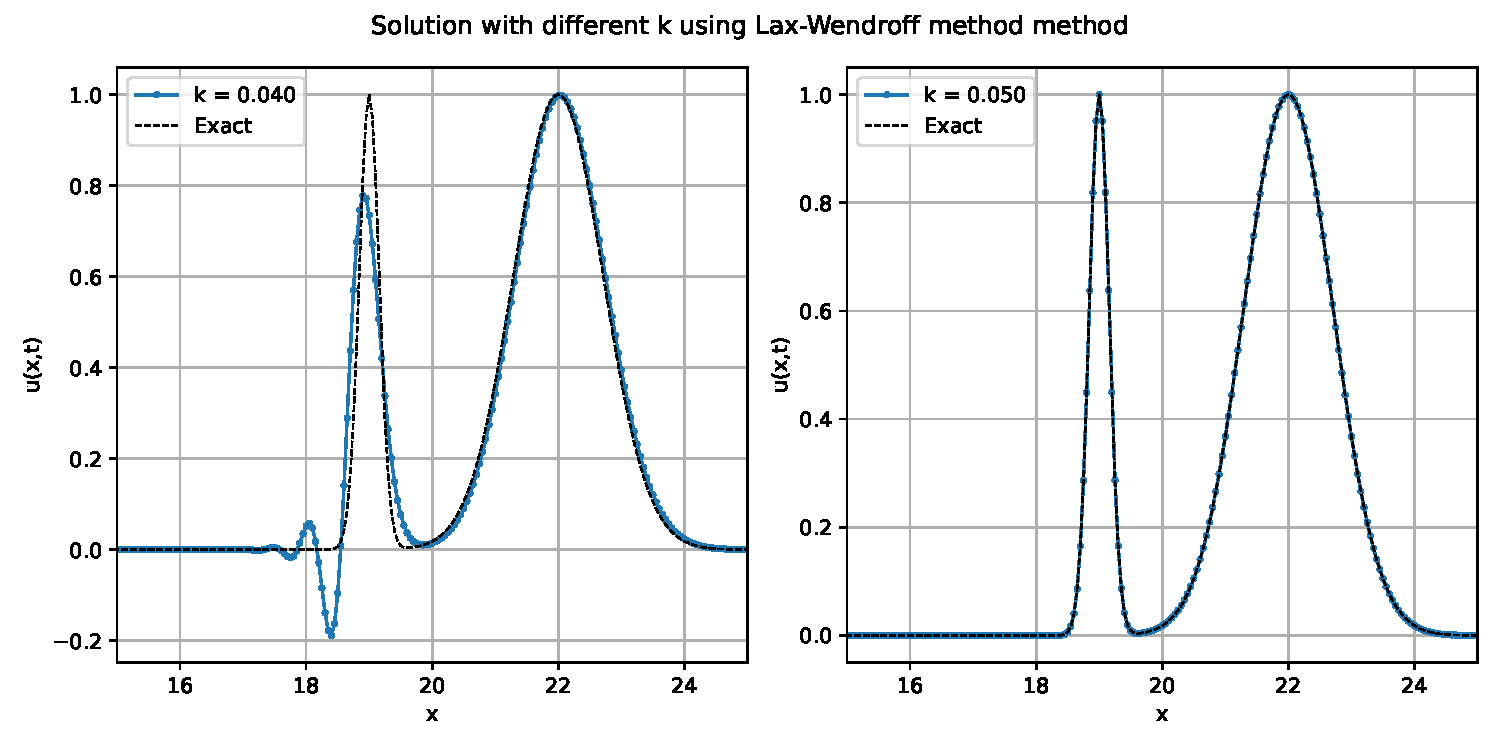
\includegraphics[width=0.67\textwidth]{figure/Lax-Wendroff_method.pdf}
    \caption{Lax-Wendroff method}
    \label{fig:Lax-Wendroff_method}
\end{figure}

\begin{figure}[htbp]
    \centering
    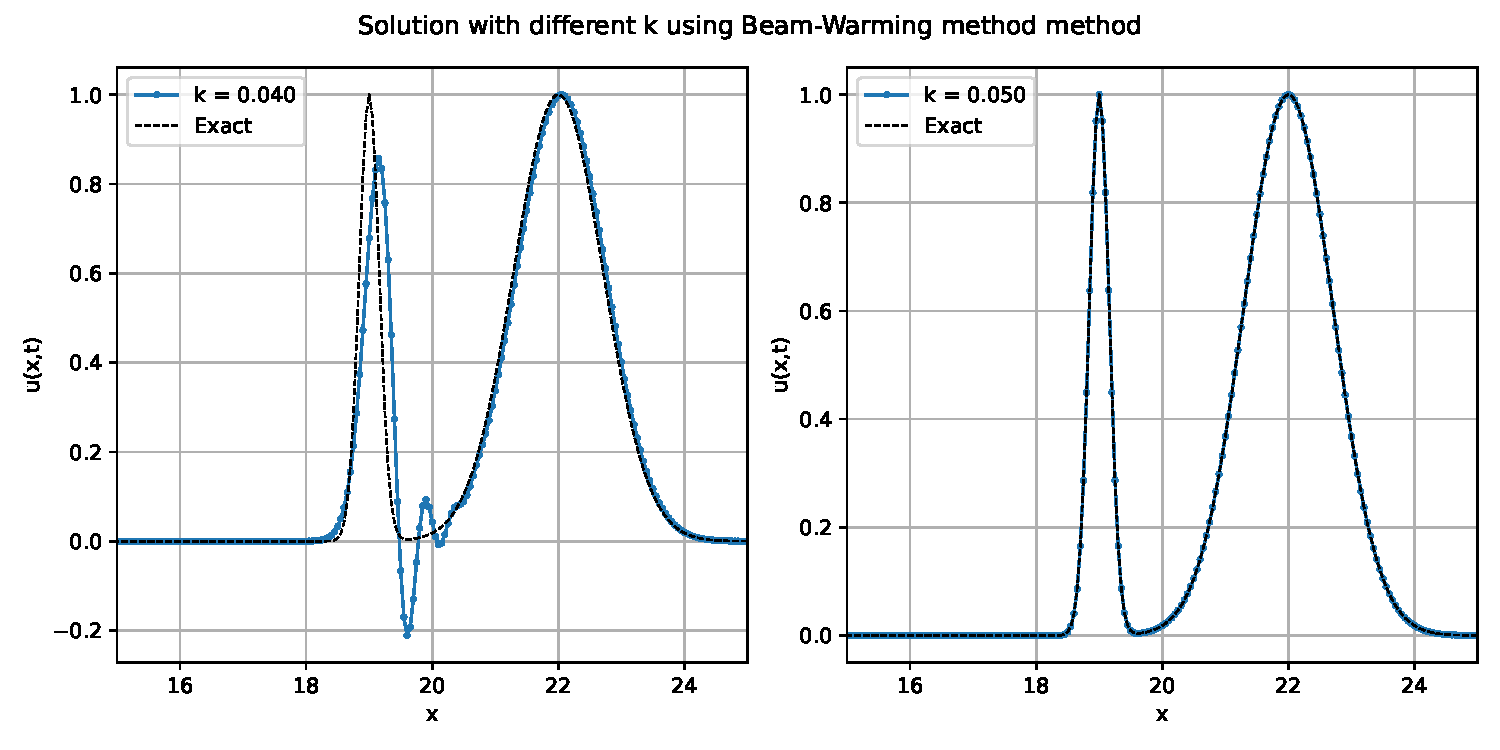
\includegraphics[width=0.67\textwidth]{figure/Beam-Warming_method.pdf}
    \caption{Beam-Warming method}
    \label{fig:Beam-Warming_method}
\end{figure}

\begin{figure}[htbp]
    \centering
    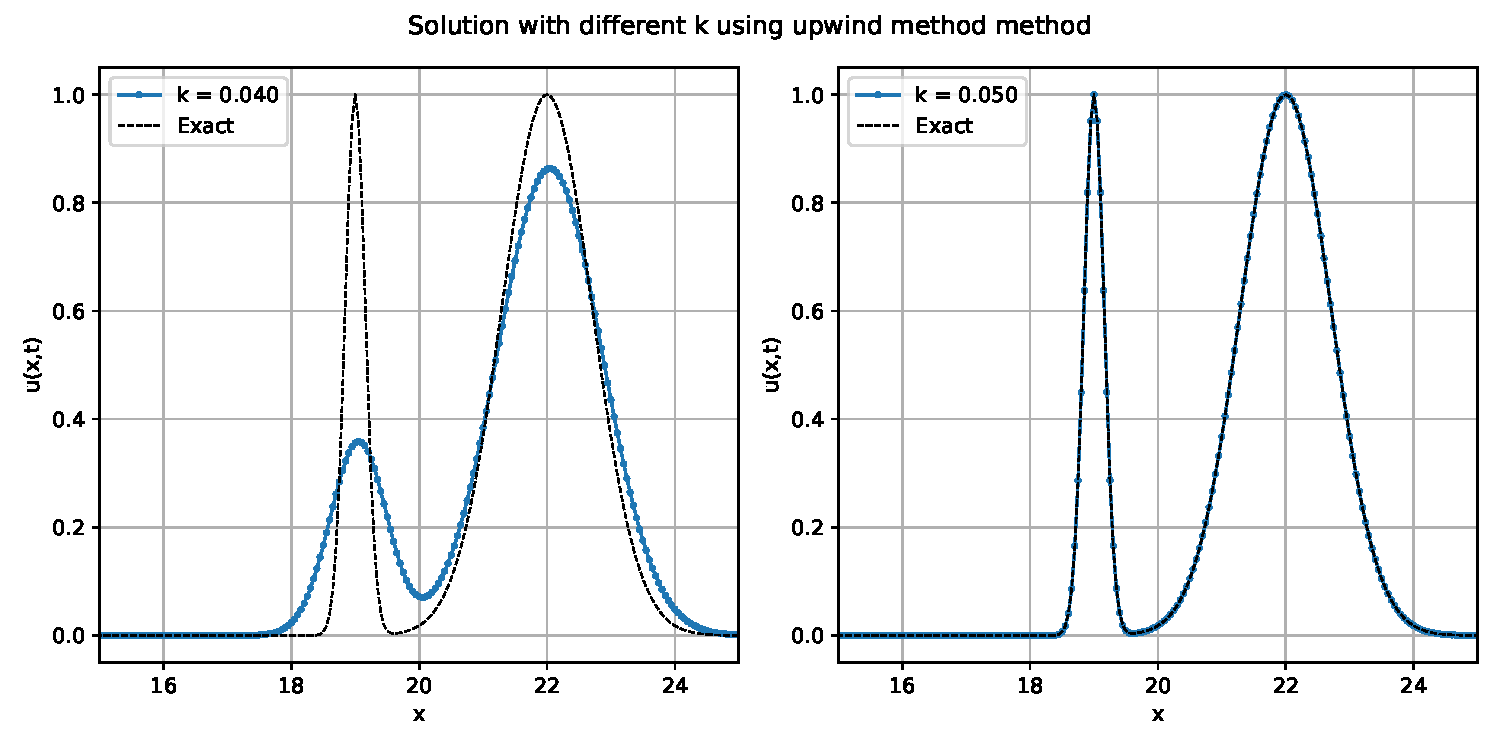
\includegraphics[width=0.67\textwidth]{figure/upwind_method.pdf}
    \caption{Upwind method}
    \label{fig:upwind_method}
\end{figure}

% ===============================================

\printbibliography

\end{document}